\documentclass[12pt]{article}

\usepackage[margin=1in]{geometry}
\usepackage[T1]{fontenc}
\usepackage[utf8]{inputenc}
\usepackage{textcomp}
\usepackage{newtxtext,newtxmath}
\usepackage{amsmath}
\usepackage{graphicx}
\usepackage{booktabs}
\usepackage{array}
\usepackage{longtable}
\usepackage{calc}
\usepackage{float}
\usepackage{caption}
\usepackage{setspace}
\usepackage{lineno}
\usepackage{xcolor}
\usepackage[round,authoryear]{natbib}
\usepackage[bookmarks=false]{hyperref}
\IfFileExists{xurl.sty}{\usepackage{xurl}}{}
\urlstyle{same}

\pagestyle{plain}
\doublespacing
\setlength{\parindent}{0pt}
\setlength{\parskip}{0pt}
\setlength{\emergencystretch}{3em}

\usepackage{titlesec}
\titleformat{\section}
  {\normalfont\large\bfseries}
  {\thesection}{0.75em}{}
\titleformat{\subsection}
  {\normalfont\normalsize\bfseries}
  {\thesubsection}{0.75em}{}
\titleformat{\subsubsection}
  {\normalfont\normalsize\itshape}
  {\thesubsubsection}{0.75em}{}
\titlespacing*{\section}{0pt}{1.2em}{0.6em}
\titlespacing*{\subsection}{0pt}{1.0em}{0.45em}
\titlespacing*{\subsubsection}{0pt}{0.8em}{0.35em}

\newcommand{\tablecaptionfontsize}{\fontsize{10pt}{12pt}\selectfont}
\newcommand{\tablefontsize}{\fontsize{9pt}{11pt}\selectfont}
\DeclareCaptionFont{captionten}{\fontsize{10pt}{12pt}\selectfont}
\captionsetup{
  font=captionten,
  labelfont=bf,
  textfont=captionten,
  justification=raggedright,
  labelsep=period,
  singlelinecheck=false
}
\newcolumntype{L}[1]{>{\tablefontsize\raggedright\arraybackslash}m{#1}}

\providecommand{\tightlist}{\setlength{\itemsep}{0pt}\setlength{\parskip}{0pt}}
\providecommand{\DOIprefix}{doi: }
\providecommand{\URLprefix}{URL: }
\providecommand{\ArXivprefix}{arXiv: }
\providecommand{\Pubmedprefix}{PMID: }
\providecommand{\doi}[1]{\href{https://doi.org/\detokenize{#1}}{\nolinkurl{#1}}}
\hypersetup{
  pdftitle={From Disease Risk to Field Action: GrapeMaster, a Model-Integrated Software Platform for Vineyard Disease Management},
  hidelinks,
  pdfcreator={LaTeX}
}

\newcommand{\figref}[1]{\hyperref[#1]{Figure~\ref*{#1}}}
\newcommand{\tabref}[2]{\hyperref[#1]{Table~#2}}
\newcommand{\manuscripttitle}{From Disease Risk to Field Action: GrapeMaster, a Model-Integrated Software Platform for Vineyard Disease Management}

\begin{document}

\linenumbers

\begin{center}
{\LARGE\setstretch{0.9}\selectfont \manuscripttitle\par}
\end{center}

\vspace{0.8em}

\begingroup
\normalsize
\setstretch{1.05}
\noindent
\mbox{Author~information~to~be~completed~before~submission}
\par
\vspace{0.7em}

\noindent
Affiliations, author order, and corresponding author details will be completed before journal submission.
\par
\endgroup

\vspace{1em}

\section*{Abstract}

Vineyard disease-management software must combine information that differs in source, timing, and operational role, including environmental observations, phenological state, disease forecasts, symptom images, advisory interaction, field operations, and treatment history. We developed GrapeMaster, a mobile and backend software platform that orchestrates these heterogeneous resources within two connected workflows. A proactive workflow assembles weather, phenology, cultivar susceptibility, and recent treatment records for disease-risk analysis, translates model output into notifications and plant-protection tasks, and returns completed treatments to subsequent risk interpretation. A post-symptomatic workflow connects image recognition with large language model (LLM)-assisted advisory interaction. The implementation combines a Flutter mobile client, a Django REST backend, relational record storage, scheduled processing, and independently deployable analytical services. Deployment records from 47 operational accounts covered 139 vineyard fields, 128 crop-management records, 3,590 notifications, 151 field-operation tasks, and 234 product records; a representative replay reconstructed the implemented risk-to-action-to-feedback sequence. Supporting component evaluations yielded 76.0\% user-visible agreement for broad phenological stages, a mean absolute error of 6.3 days for downy mildew first-infection timing, and class-wise F1-scores of 0.926--0.998 for image recognition. LLM advisory quality was not independently evaluated. GrapeMaster demonstrates how predictive, diagnostic, advisory, and operational services can be integrated into a persistent field-management application rather than delivered as isolated analytical outputs.

\noindent\textbf{Keywords:} grapevine; disease management; software architecture; model integration; decision support system; large language model; treatment feedback

\section{Introduction}\label{introduction}

Grapevine disease management requires repeated decisions under changing environmental, biological, and operational conditions. In humid subtropical production regions, high temperature, persistent rainfall, humidity, and leaf wetness can increase the frequency and severity of downy mildew infection \citep{gesslerPlasmoparaViticolaReview2011,yuEffectsRainShelter2017}. Growers must interpret current weather and host development, anticipate infection, inspect symptoms, select control measures, and account for recent treatments. When these decisions depend primarily on experience, paper records, or informal information sources, relevant evidence is difficult to combine and review \citep{tummersObstaclesFeaturesFarm2019,yaoInfluenceInformationSources2025}. Inappropriate fungicide use can then increase costs and environmental pressure without improving control \citep{oliverFungicideUsePatterns2023,zubrodFungicidesOverlookedPesticide2019}. Digital support must therefore address not only disease prediction, but also the continuity of information from risk recognition to field action.

Several analytical technologies support different parts of this process. Weather-driven disease models characterize infection conditions and treatment timing \citep{rossiMechanisticModelSimulating2008,caffiEvaluationDynamicModel2011}; phenology models describe host development and susceptible periods \citep{parkerGeneralPhenologicalModel2011a,wangAssessingGrapevinePhenological2020}; image-recognition models provide post-symptomatic classification; and large language models (LLMs) can support natural-language interpretation and advisory interaction \citep{raiAdvancingSitespecificDisease2026,yanCDIPChatGLM3DualmodelApproach2025}. These components differ in input type, temporal resolution, execution pattern, and user role. A scheduled disease forecast, an image-classification request, and an interactive advisory exchange therefore cannot be integrated by merely displaying their outputs on the same screen. They require software mechanisms for assembling context, invoking services, storing requests and responses, presenting results, and relating management actions to subsequent analysis.

Agricultural decision-support systems increasingly combine monitoring, modeling, communication, and farm-management functions \citep{fountasFarmManagementInformation2015,zhaiDecisionSupportSystems2020}. In viticulture, vite.net connected vineyard monitoring with model-based decision support and bidirectional communication, while MISFITS-DSS delivered regional downy mildew assessment for public plant-protection services \citep{rossiAddressingImplementationProblem2014,bregaglioPublicDecisionSupport2022}. Broader agricultural platforms integrate sensing, multimodal data, analytical services, and user interaction \citep{bakirScalableEndtoendIoT2026,chenAgriculturalAutonomousDecisionmaking2026}. These systems establish the value of integration, but they also reveal a continuing software challenge: heterogeneous analytical services must be coordinated with persistent field context, user-facing events, executable operations, treatment records, and later review. The relevant gap is therefore not the absence of integrated platforms, but the need for explicit and reproducible model-to-management orchestration.

For vineyard disease management, such orchestration requires several capabilities. The software must preserve stable field identity while retaining time-dependent environmental, crop, analytical, and operational records; construct model requests from multiple data sources; translate analytical outputs into warnings and management functions; and incorporate completed treatments into later risk interpretation. It must also support two complementary decision pathways: a proactive pathway based on weather, phenology, and disease forecasting, and a post-symptomatic pathway based on images and advisory interaction. These requirements define an agricultural computing problem in which the contribution lies in the relationships among analytical services, application logic, persistent records, and field operations rather than in any individual model alone \citep{mccownLocatingAgriculturalDecision2002,roseDecisionSupportTools2016,romera2024digitalization}.

To address this problem, we developed GrapeMaster, a model-integrated software platform for vineyard disease management. GrapeMaster combines a Flutter mobile client, a Django REST backend, relational record storage, scheduled processing, and independently deployable analytical services. The study makes four contributions: (1) an integrated computing framework that combines predictive, diagnostic, advisory, and operational functions; (2) a model-to-application mechanism through which the backend assembles inputs, invokes analytical services, persists their outputs, and translates results into user-facing information; (3) a management-feedback mechanism that transforms completed treatment records into inputs for subsequent disease-risk interpretation; and (4) a deployed mobile and backend implementation demonstrated through operational records, an end-to-end workflow replay, and bounded validation of analytical components. Crop-season identifiers are used as one database mechanism for organizing time-dependent records, but the primary contribution is the orchestration of disease-management intelligence and field action.

\section{Materials and methods}\label{materials-and-methods}

\subsection{System objectives and usage scenarios}\label{system-objectives}

GrapeMaster was designed for growers and technical advisors who need to review field conditions, anticipate disease risk, record plant-protection operations, diagnose visible symptoms, and retrieve previous management information through a mobile application. Two usage scenarios guided the software design. The proactive scenario begins with field configuration and scheduled acquisition of environmental data. Weather and phenological state are combined with cultivar susceptibility and treatment history for disease-risk analysis; the resulting information is delivered through the mobile application and retained with notifications, tasks, and applied products. The post-symptomatic scenario begins with an image or user question and connects image recognition with LLM-assisted advisory interaction.

These scenarios were translated into six software requirements (Table~\ref{tab:system_requirements}). Heterogeneous data and model results had to remain associated with the relevant field-management context; analytical services had to be callable through explicit interfaces; scheduled and user-triggered computations had to coexist; model results had to be transformed into reviewable application information; field-operation records had to be available to later analytical requests; and diagnostic and advisory functions had to remain distinguishable from regulated plant-protection decisions.

\begin{table}[H]
\centering
\caption{Management needs, software requirements, and implemented GrapeMaster mechanisms.}
\label{tab:system_requirements}
\tablefontsize
\begin{tabular}{@{}p{0.25\linewidth} p{0.34\linewidth} p{0.33\linewidth}@{}}
\toprule
Management need & Software requirement & Implemented mechanism \\
\midrule
Maintain current field state & Combine persistent field attributes with time-dependent weather, phenology, risk, and management records & Relational field and crop-management records linked by identifiers and timestamps \\
Anticipate infection & Assemble weather, host stage, susceptibility, disease target, and treatment history & Backend disease-model request construction and scheduled service invocation \\
Deliver actionable information & Convert analytical output into user-facing events and work items & Risk displays, notifications, reminders, and task interfaces \\
Account for intervention & Make completed product applications available to subsequent analysis & Task-to-product linkage and treatment-history transformation \\
Interpret visible symptoms & Submit images and retain diagnostic output & Hosted image-recognition service and image-analysis records \\
Support explanation and interaction & Exchange questions and diagnostic or management context with an advisory model & LLM service interface, advisory sessions, and message records \\
\bottomrule
\end{tabular}
\end{table}

\subsection{Overall software architecture}\label{system-architecture}

GrapeMaster comprises a mobile application, an application backend, persistent data storage, scheduled processing, and analytical services (Figure~\ref{fig:implementation_overview}). The Flutter client provides field mapping, weather and phenology views, disease-risk timelines, notifications, tasks, product records, image upload, and advisory interaction. It communicates with the backend through HTTP APIs and persistent connections used by message-oriented functions.

The Django REST backend owns application identifiers and business records. It manages authentication, API routing, field and crop records, reference tables, notification and task logic, product records, analytical request-response payloads, and scheduled jobs. PostgreSQL stores relational objects, while the backend coordinates calls to configured weather, disease-model, image-recognition, and advisory services. Analytical services are separated from presentation logic: the backend or mobile client invokes them through service endpoints and translates their responses into application records and views. This separation allows a service to be recalibrated or replaced while preserving the surrounding user workflow, provided that the interface contract is maintained.

\begin{figure}[H]
\centering
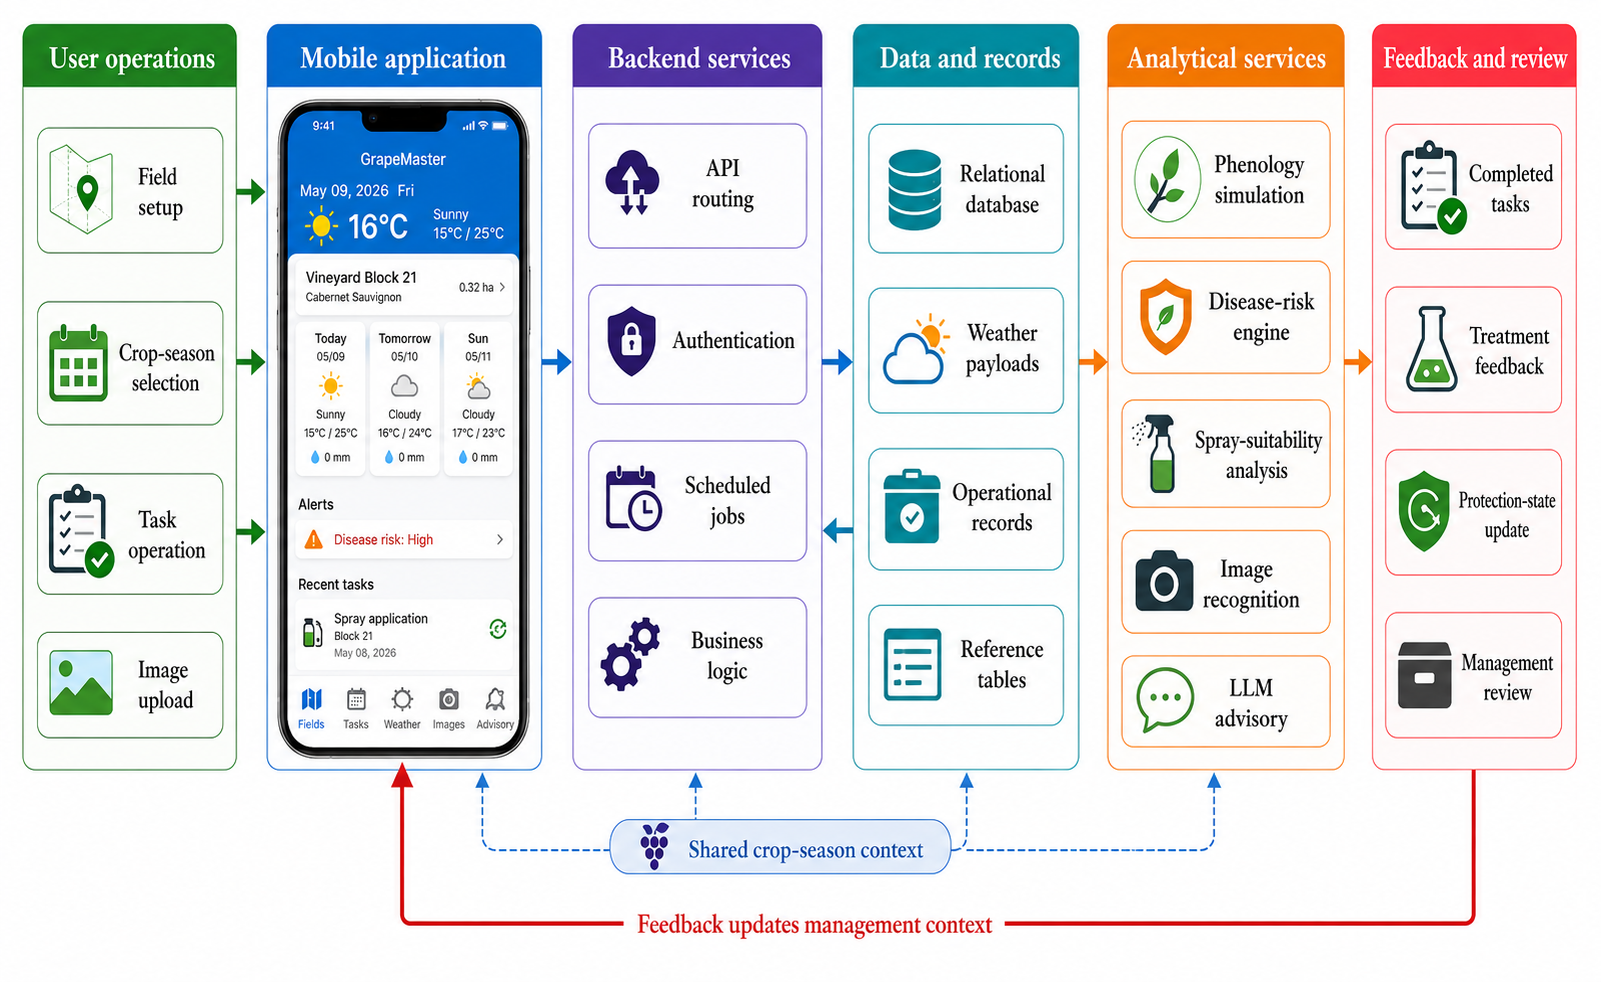
\includegraphics[width=\linewidth]{../fig/figure3_new.png}
\caption[Overall software architecture of GrapeMaster]{Overall software architecture of GrapeMaster. User operations enter through the mobile application; backend services coordinate persistent records, scheduled jobs, and analytical-service calls; completed operations update the management information available to later analysis. The crop-management identifier shown at the bottom is a data-linkage mechanism rather than a separate analytical layer.}
\label{fig:implementation_overview}
\end{figure}

\subsection{Data organization and workflow coordination}\label{data-organization}

The data model separates a persistent vineyard field from a crop-management record attached to that field. The field retains location, boundary, area, and other stable attributes. The crop-management record carries a UUID and links cultivar, cultivation method, vine age, and field context to time-dependent records. In the implemented codebase this object is named \texttt{CropSeason} in the backend and \texttt{Crop} in the frontend; it functions as an execution and retrieval key rather than as the conceptual contribution of the platform.

Weather, phenology, disease-risk, and model request-response records are stored against this management key. Notifications and field-operation tasks also retain field, user, or crop context as implemented by their respective objects. Fungicide and pesticide products are linked directly to plant-protection tasks through task identifiers. Image analyses, disease reports, notes, advisory sessions, and messages use account, field, crop, image, or message identifiers depending on the function. Consequently, some relationships are direct foreign-key links, whereas others are contextual associations recovered through a shared field, crop, or user context. The manuscript distinguishes these relationships and does not infer a direct notification-to-task causal link where the schema stores only shared context.

The backend coordinates workflow state by retrieving the records needed for a particular operation. For a disease-model call, it assembles environmental, phenological, cultivar, disease-target, and recent treatment information. For mobile presentation, it combines stored analytical results with current notifications, tasks, and historical records. For advisory interaction, it retains the user query and returned message with the available account, image, or field context. Supplementary Figure S1 and Supplementary Tables S2 and S6 provide the extended entity and record definitions.

\subsection{Environmental and phenological information}\label{weather-and-phenology-processing}

Field coordinates are used by scheduled backend jobs to request historical and forecast payloads from the configured weather service. The backend transforms daily temperature series for phenology processing, hourly variables for disease-risk analysis, and short-term weather variables for spray-suitability display. Date alignment and missing-value handling are completed before analytical requests are assembled. The provider is configured outside the client; the deployed provider and endpoint version are therefore release-level dependencies rather than properties of the user interface.

The phenology component receives cultivar or crop metadata and daily temperature data and returns a date-aligned broad-stage sequence. Its output supports three software functions: presentation of crop development in the mobile workspace, interpretation of host susceptibility in the disease-risk service, and timing information for management tasks. The current study used a Guangxi-calibrated temperature-driven phenology workflow rather than proposing a new phenology model \citep{parkerGeneralPhenologicalModel2011a,wangAssessingGrapevinePhenological2020}.

\subsection{Disease-model integration}\label{disease-model-integration}

The disease-risk service is integrated through a request-response interface (Figure~\ref{fig:disease_risk_engine_structure}). A backend job or application event initiates request construction. The request contains date-aligned weather variables, phenological stages, cultivar susceptibility, the target disease, and recent fungicide applications. The independently deployable disease service then evaluates daily infection conditions, derives field-risk and protection states, and returns date-aligned risk information, recommendations, and treatment-window information. Both request and response payloads are retained by the backend so that the analytical state presented to the user can be examined with its inputs.

For the reported Guangxi configuration, the principal validated pathway was the FSIM-S downy mildew first-infection module. Its infection-process logic was derived from published downy mildew models and calibrated with Guangxi observations \citep{rossiMechanisticModelSimulating2008,caffiModelPredictingPrimary2009c,caffiEvaluationDynamicModel2011,brischettoWeatherDrivenModelPredicting2021}. The service architecture can expose additional disease pathways, but the results in this paper support only the downy mildew first-infection configuration unless separate validation is reported. Extensive equations and parameters are provided in Supplementary Table S1; the main text focuses on the software interface and use of model output.

\begin{figure}[H]
\centering
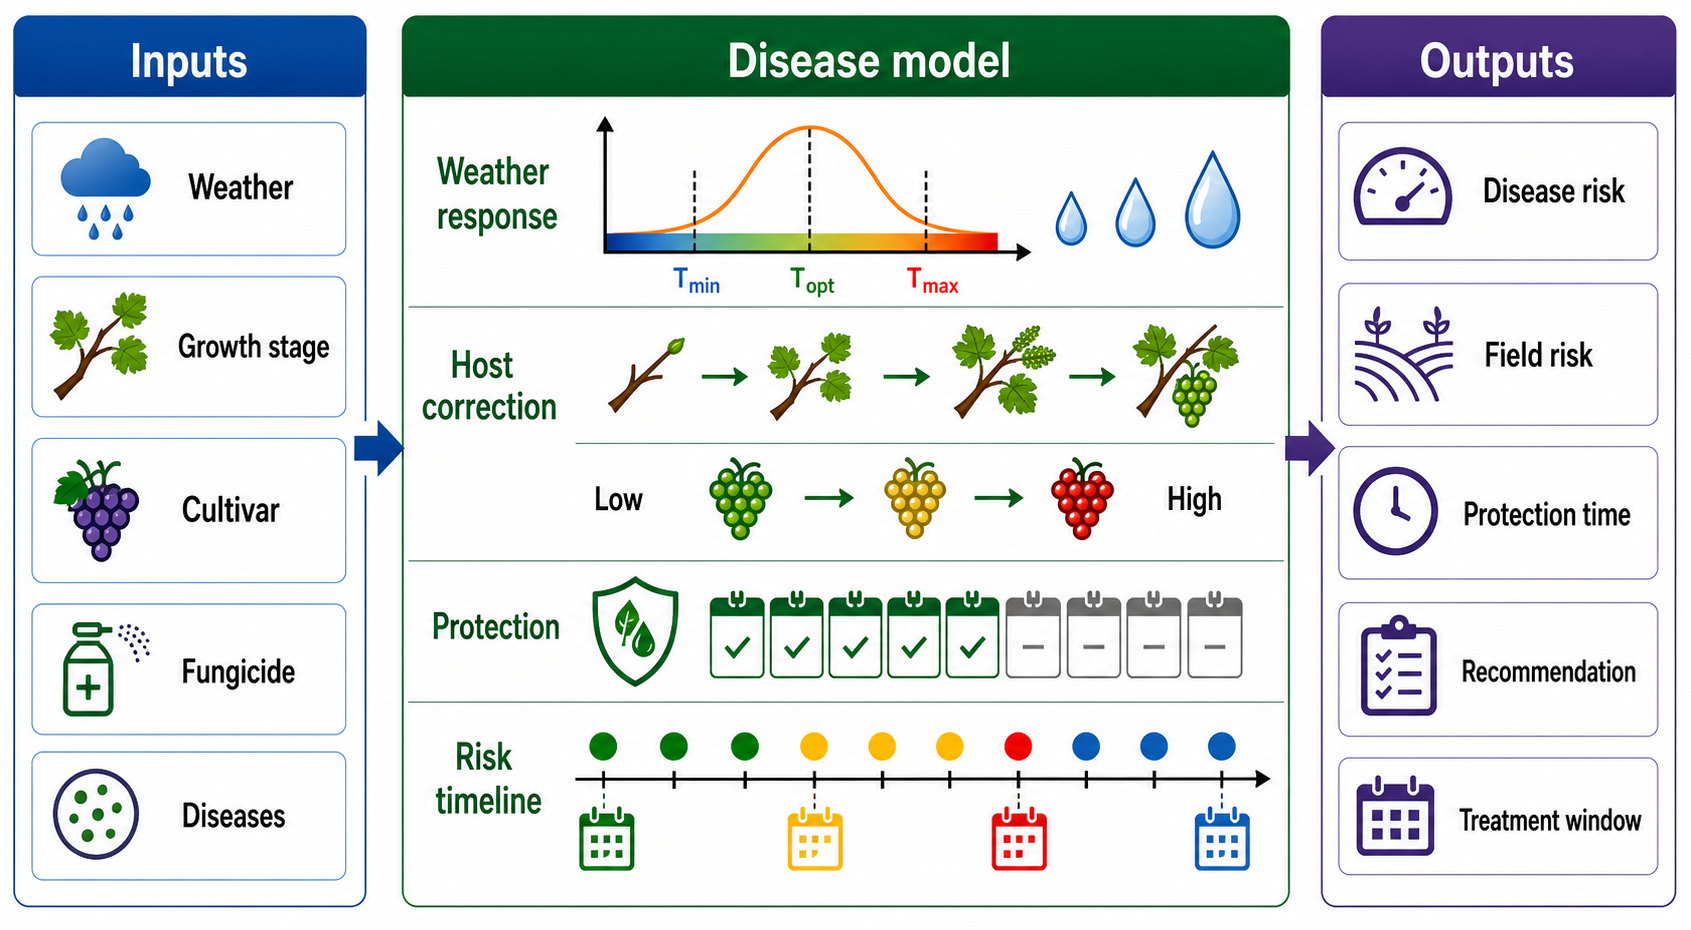
\includegraphics[width=\linewidth]{../fig/fig03_disease_model_workflow.png}
\caption[Disease-model integration in GrapeMaster]{Disease-model integration in GrapeMaster. The backend assembles weather, host stage, cultivar susceptibility, recent fungicide information, and disease target; the service returns disease risk, field risk, protection time, recommendations, and treatment windows for storage and presentation.}
\label{fig:disease_risk_engine_structure}
\end{figure}

\subsection{Field operations and treatment feedback}\label{disease-risk-service-and-treatment-feedback-workflow}

Disease-risk responses are transformed into application information rather than displayed as unconnected model files. Risk states and treatment windows are presented in date-aligned views, and associated warning or management events can be delivered as notifications. Users create plant-protection tasks within the same field-management context and record execution date, selected products, dosage-related information, treated area, and water volume. Notification and task records may share context without a direct causal foreign key; product records, however, are linked directly to their tasks.

When a plant-protection task contains a fungicide record, the backend serializer translates the target, application date, and protection-duration information into the \texttt{applied\_fungicides} structure accepted by the disease service. The stored disease-model request is updated, and applicable task operations initiate a subsequent service call. This mechanism allows later risk interpretation to account for recent treatment history. It represents a software feedback operation, not a claim that the platform measured biological efficacy. Protection duration remains an analytical assumption influenced by product properties, host growth, rainfall, and disease pressure \citep{caffiFungicideModelsAre2018,oliverFungicideUsePatterns2023,warnekeEffectFungicideMobility2020}.

\subsection{Image-recognition and LLM advisory integration}\label{image-recognition-and-advisory-services}

The post-symptomatic workflow separates visual classification from language-based interaction (Figure~\ref{fig:image_advisory_workflow}). The mobile client submits a user-selected symptom image to a hosted recognition service. The returned disease or healthy class and confidence value are displayed and retained as image-analysis records. In the current application this branch covers several grape disease categories rather than only downy mildew.

The advisory interface sends user questions and available diagnostic or management context to a separately hosted LLM service and presents the returned text as a conversational response. Advisory sessions and messages are retained for later retrieval. The integration follows the published CDIP-ChatGLM3 approach, which couples a visual disease classifier with a fine-tuned ChatGLM3-based advisory component \citep{yanCDIPChatGLM3DualmodelApproach2025}. The contribution claimed here is the software interface and workflow integration; the model checkpoint, service version, prompt or context-construction rules, and deployment configuration are version-specific release metadata. Advisory output is informational and does not replace expert diagnosis, pesticide labels, or regulated plant-protection decisions.

\begin{figure}[H]
\centering

\includegraphics[width=\linewidth]{../fig/fig13_image_assistance_workflow.png}
\caption[Image-recognition and LLM-assisted advisory workflow]{Post-symptomatic image-recognition and LLM-assisted advisory workflow in GrapeMaster. The visual service returns a disease class and confidence, while the advisory service supports contextual follow-up questions and management-oriented explanations. LLM, large language model.}
\label{fig:image_advisory_workflow}
\end{figure}

\subsection{Software implementation, deployment, and supporting evidence}\label{implementation}

The mobile application was implemented in Flutter. The application backend used Django 4.2 and Django REST Framework with PostgreSQL storage, scheduled background jobs, and message-oriented connections. The disease-risk component was deployed as a separate FastAPI service. Image recognition and advisory were invoked through separately hosted service endpoints. Table~\ref{tab:module_provenance} summarizes the role and evidence boundary of each integrated component.

\begin{table}[H]
\centering
\caption{Integrated GrapeMaster components, software roles, and evidence reported in this study.}
\label{tab:module_provenance}
\tablefontsize
\begin{tabular}{@{}p{0.19\linewidth} p{0.27\linewidth} p{0.28\linewidth} p{0.18\linewidth}@{}}
\toprule
Component & Interface and invocation & Application role & Supporting evidence \\
\midrule
Weather and phenology & Scheduled backend acquisition and processing & Environmental and host-development state for display and modeling & Deployment payloads and phenology validation \\
Disease-risk service & Backend-generated request to an independent service & Pre-symptomatic risk, protection-state, and treatment-window information & Stored request-response records and downy mildew validation \\
Task and treatment services & Mobile/backend business APIs and relational task-product records & Operation planning, execution, and treatment feedback & Deployment records and workflow replay \\
Image recognition & User-triggered hosted inference endpoint & Post-symptomatic class and confidence output & Image-analysis records and offline image validation \\
LLM advisory & User-triggered hosted conversational endpoint & Contextual explanation and advisory interaction & Message records; advisory quality not independently evaluated \\
\bottomrule
\end{tabular}
\end{table}

Operational records exported from the deployed backend were used to demonstrate that the intended objects and connections existed in practice. Accounts were deduplicated by backend user key; accounts without both a field and crop-management record were excluded from the operational set. Field and crop records were retained when they contained valid identifiers and relationships. Weather, phenology, disease-risk, request-response, notification, task, product, image, advisory, note, report, and forum records were then counted within the retained set. A representative case containing environmental, analytical, event, task, and product records was selected to replay the proactive workflow. These procedures assessed implementation coverage and reconstructability, not usability, adoption, disease-control efficacy, pesticide reduction, or economic performance.

Analytical components were evaluated independently of the deployment demonstration. Broad-stage phenology used 151 valid observations from six Guangxi site-years. Downy mildew evaluation used first-infection observations from Guangxi vineyards. Image recognition used a labeled grape disease image dataset. Exact agreement, transition-window agreement, and mean absolute stage distance were used for phenology; mean absolute error (MAE) and root mean square error (RMSE) were used for first-infection timing; and class-wise F1-score was used for image recognition. LLM advisory quality was not independently evaluated.

\section{Results}\label{results}

\subsection{Implemented GrapeMaster application}\label{features-and-functionalities}

The implemented application provided field creation and boundary editing, crop configuration, weather and spray-suitability views, phenology and risk summaries, notifications, task and product management, image upload, and advisory interaction. Field configuration established the spatial context used by scheduled environmental requests and later records (Figure~\ref{fig:field_crop_season_entry_points}). The main workspace combined near-term weather, spray suitability, crop development, and current risk information without requiring users to open separate analytical tools (Figure~\ref{fig:weather_phenology_interfaces_result}).

\begin{figure}[H]
\centering
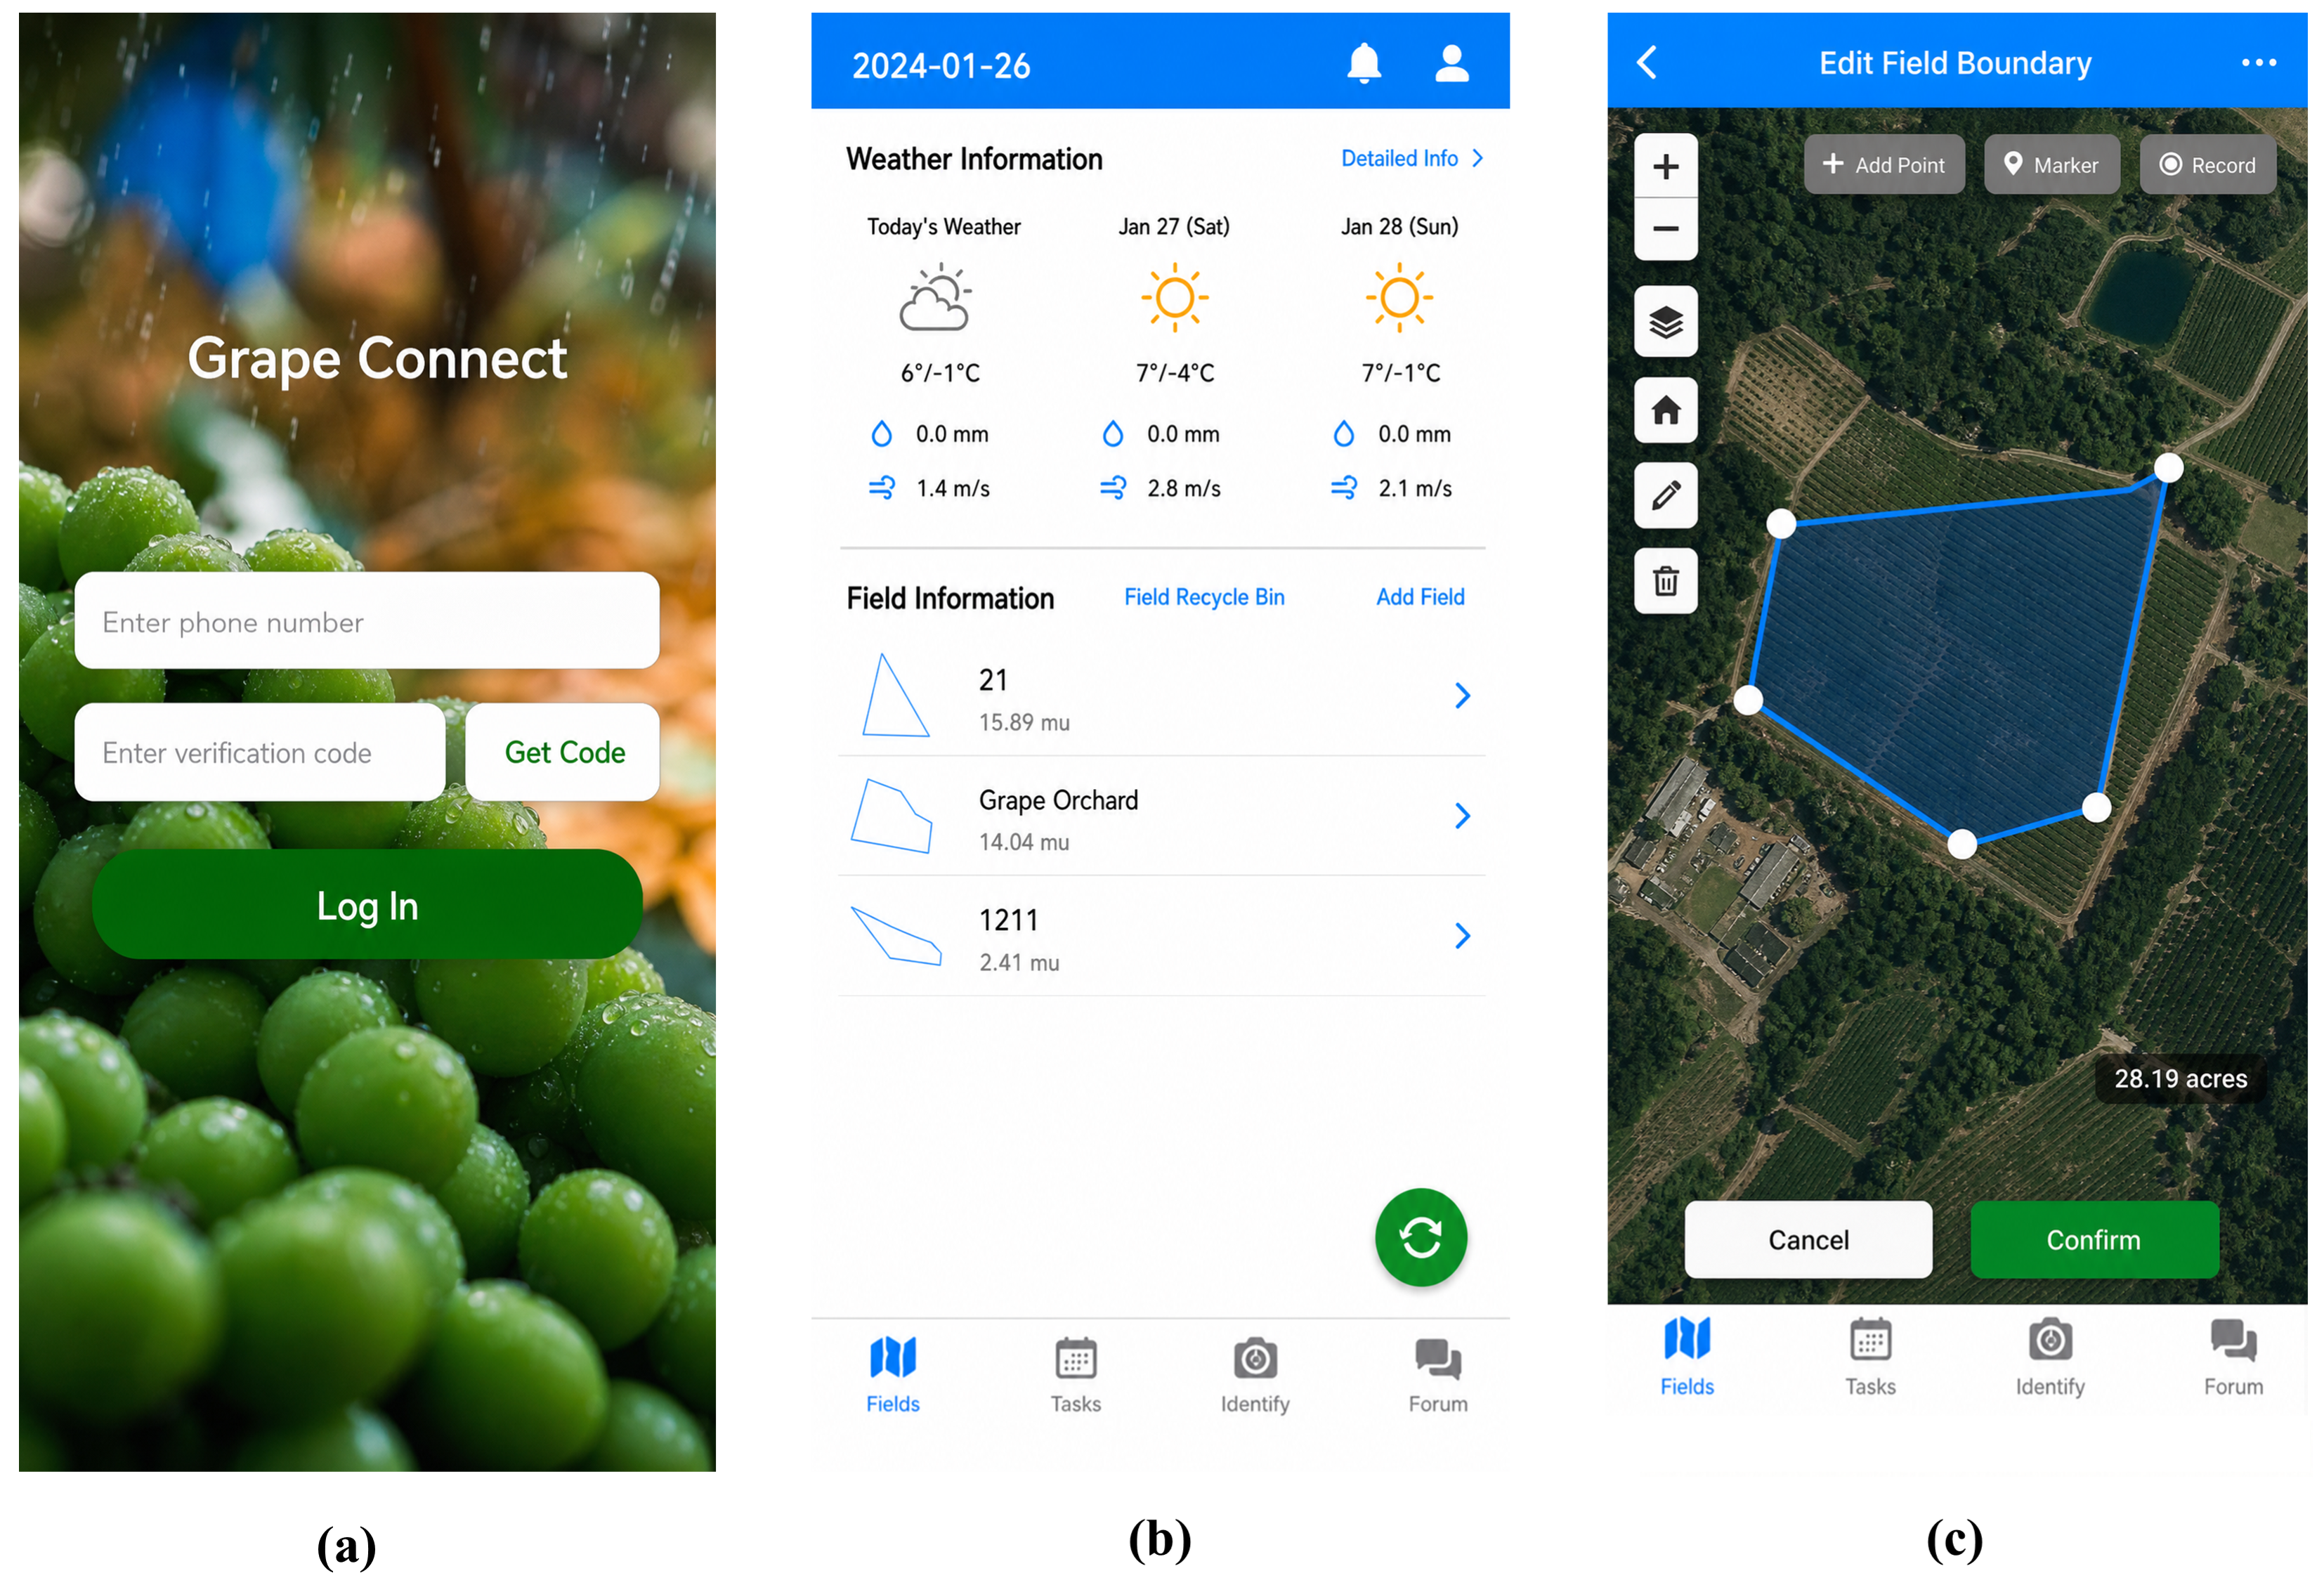
\includegraphics[width=\linewidth]{../fig/field_management_interfaces.png}
\caption[Field configuration in the mobile application]{Representative mobile entry points for authentication, field selection, and vineyard-boundary editing in GrapeMaster.}
\label{fig:field_crop_season_entry_points}
\end{figure}

\begin{figure}[H]
\centering
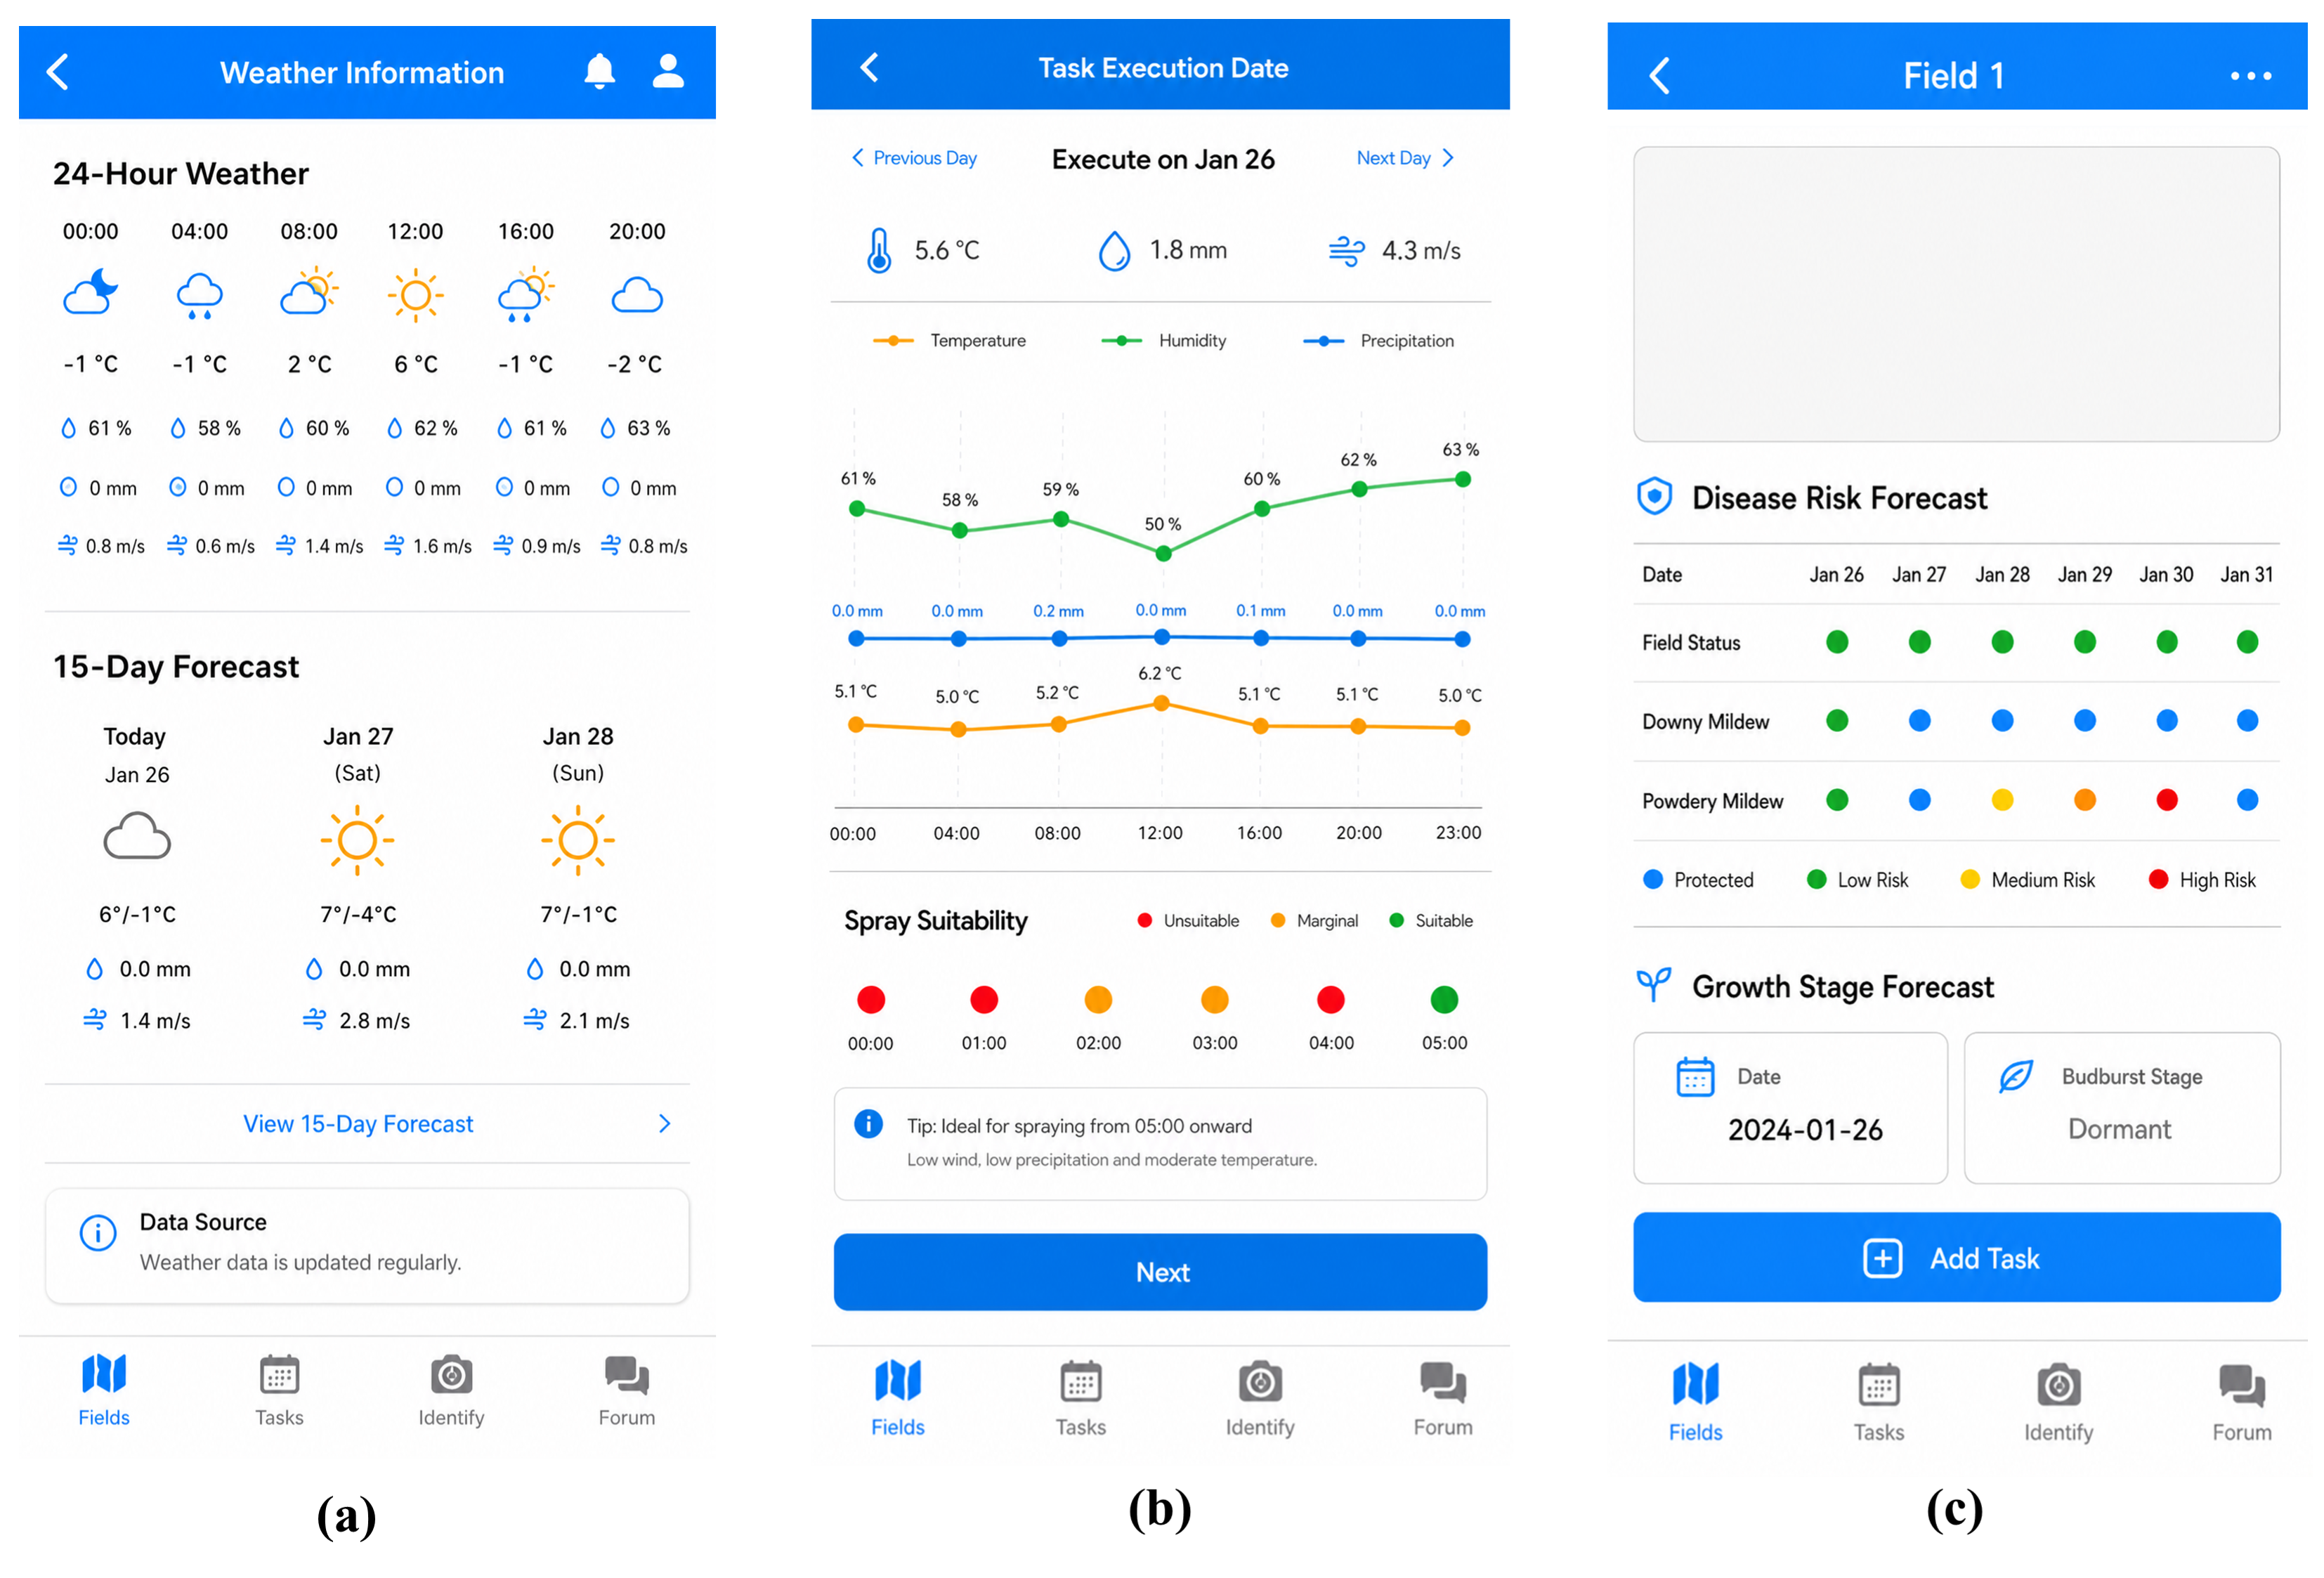
\includegraphics[width=\linewidth]{../fig/weather_phenology_interfaces.png}
\caption[Environmental and phenological information in GrapeMaster]{Environmental and phenological information in GrapeMaster. (a) Field-specific near-term weather. (b) Hourly spray-suitability information. (c) Field-risk and phenological-stage summaries in the selected management workspace.}
\label{fig:weather_phenology_interfaces_result}
\end{figure}

\subsection{Proactive risk-to-action-to-feedback workflow}\label{risk-display-and-notification-delivery}\label{task-execution-and-product-feedback}

The proactive workflow connected model output with field-management functions. Date-aligned views displayed disease and field-risk states and showed how recorded fungicide applications changed protection-state interpretation (Figure~\ref{fig:disease_risk_timeline_result}). Generated disease or management events were delivered through alert dialogs and retained in the notification archive (Figure~\ref{fig:alert_notification_interfaces_result}). Within the corresponding field context, users could create tasks, select fungicide or pesticide products, record task status, and calculate tank-mixing information (Figure~\ref{fig:task_management_interfaces_result}).

After a product was recorded for a plant-protection task, its treatment information was available to the backend transformation described in Section~\ref{disease-risk-service-and-treatment-feedback-workflow}. The resulting workflow therefore extended from risk calculation to user-facing delivery, operation recording, and treatment-aware recalculation. The implementation supports this functional sequence, although the present schema does not establish a direct causal foreign key from a particular notification to a particular task.

\begin{figure}[H]
\centering
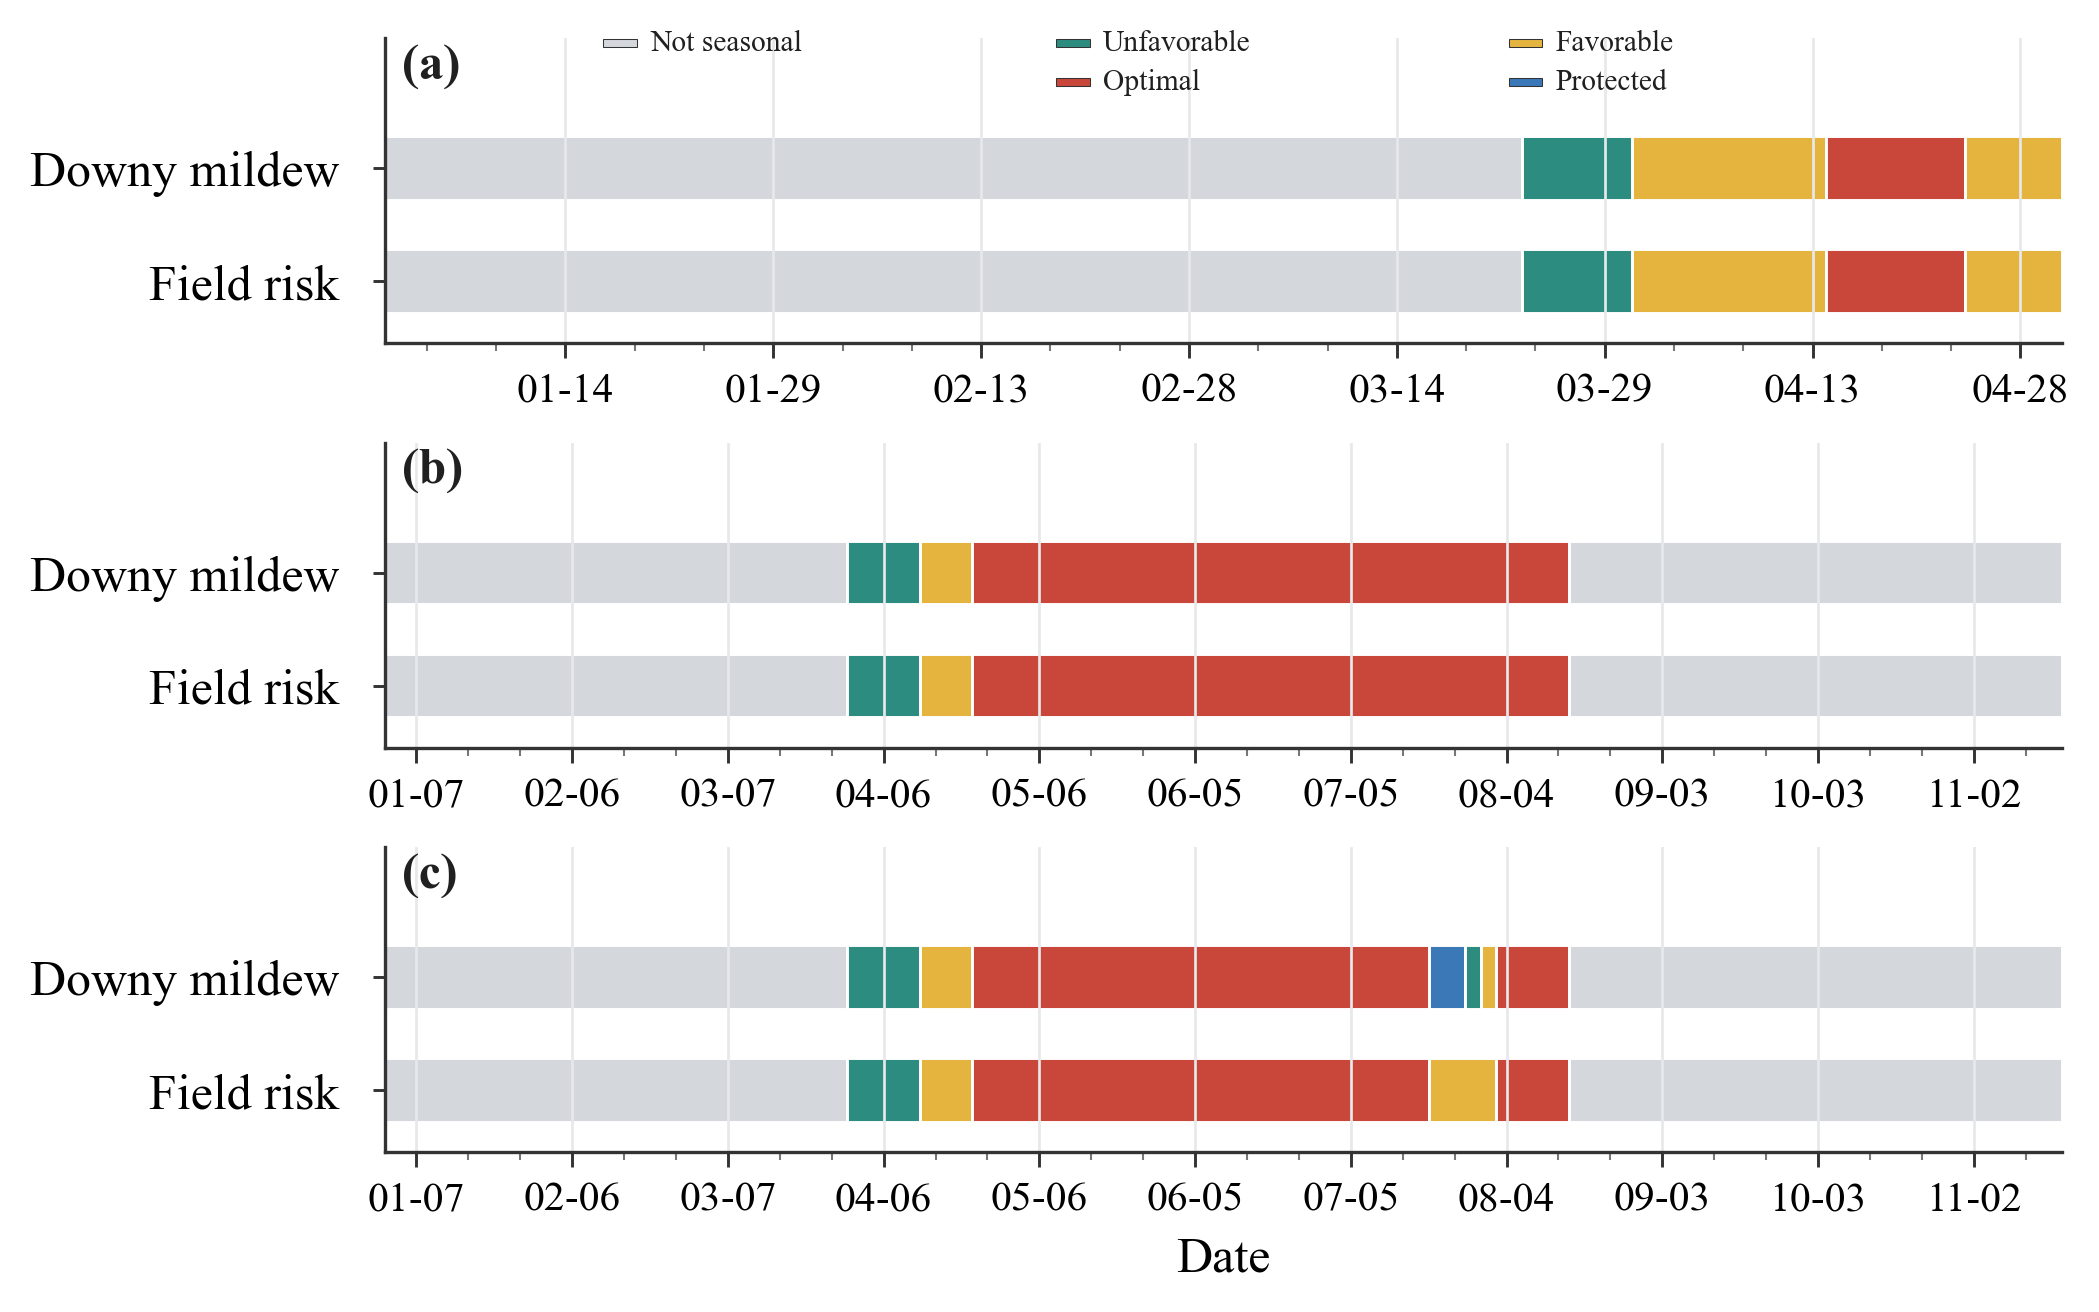
\includegraphics[width=\linewidth]{../fig/disease_risk_timeline_downy_field.png}
\caption[Disease-risk timeline and treatment-aware update]{Disease-risk timeline and treatment-aware update in GrapeMaster. (a) Date-aligned downy mildew and field-risk states for Mingyang in 2024. (b) Risk interpretation without fungicide feedback. (c) The corresponding protection-state update when fungicide records are included.}
\label{fig:disease_risk_timeline_result}
\end{figure}

\begin{figure}[H]
\centering
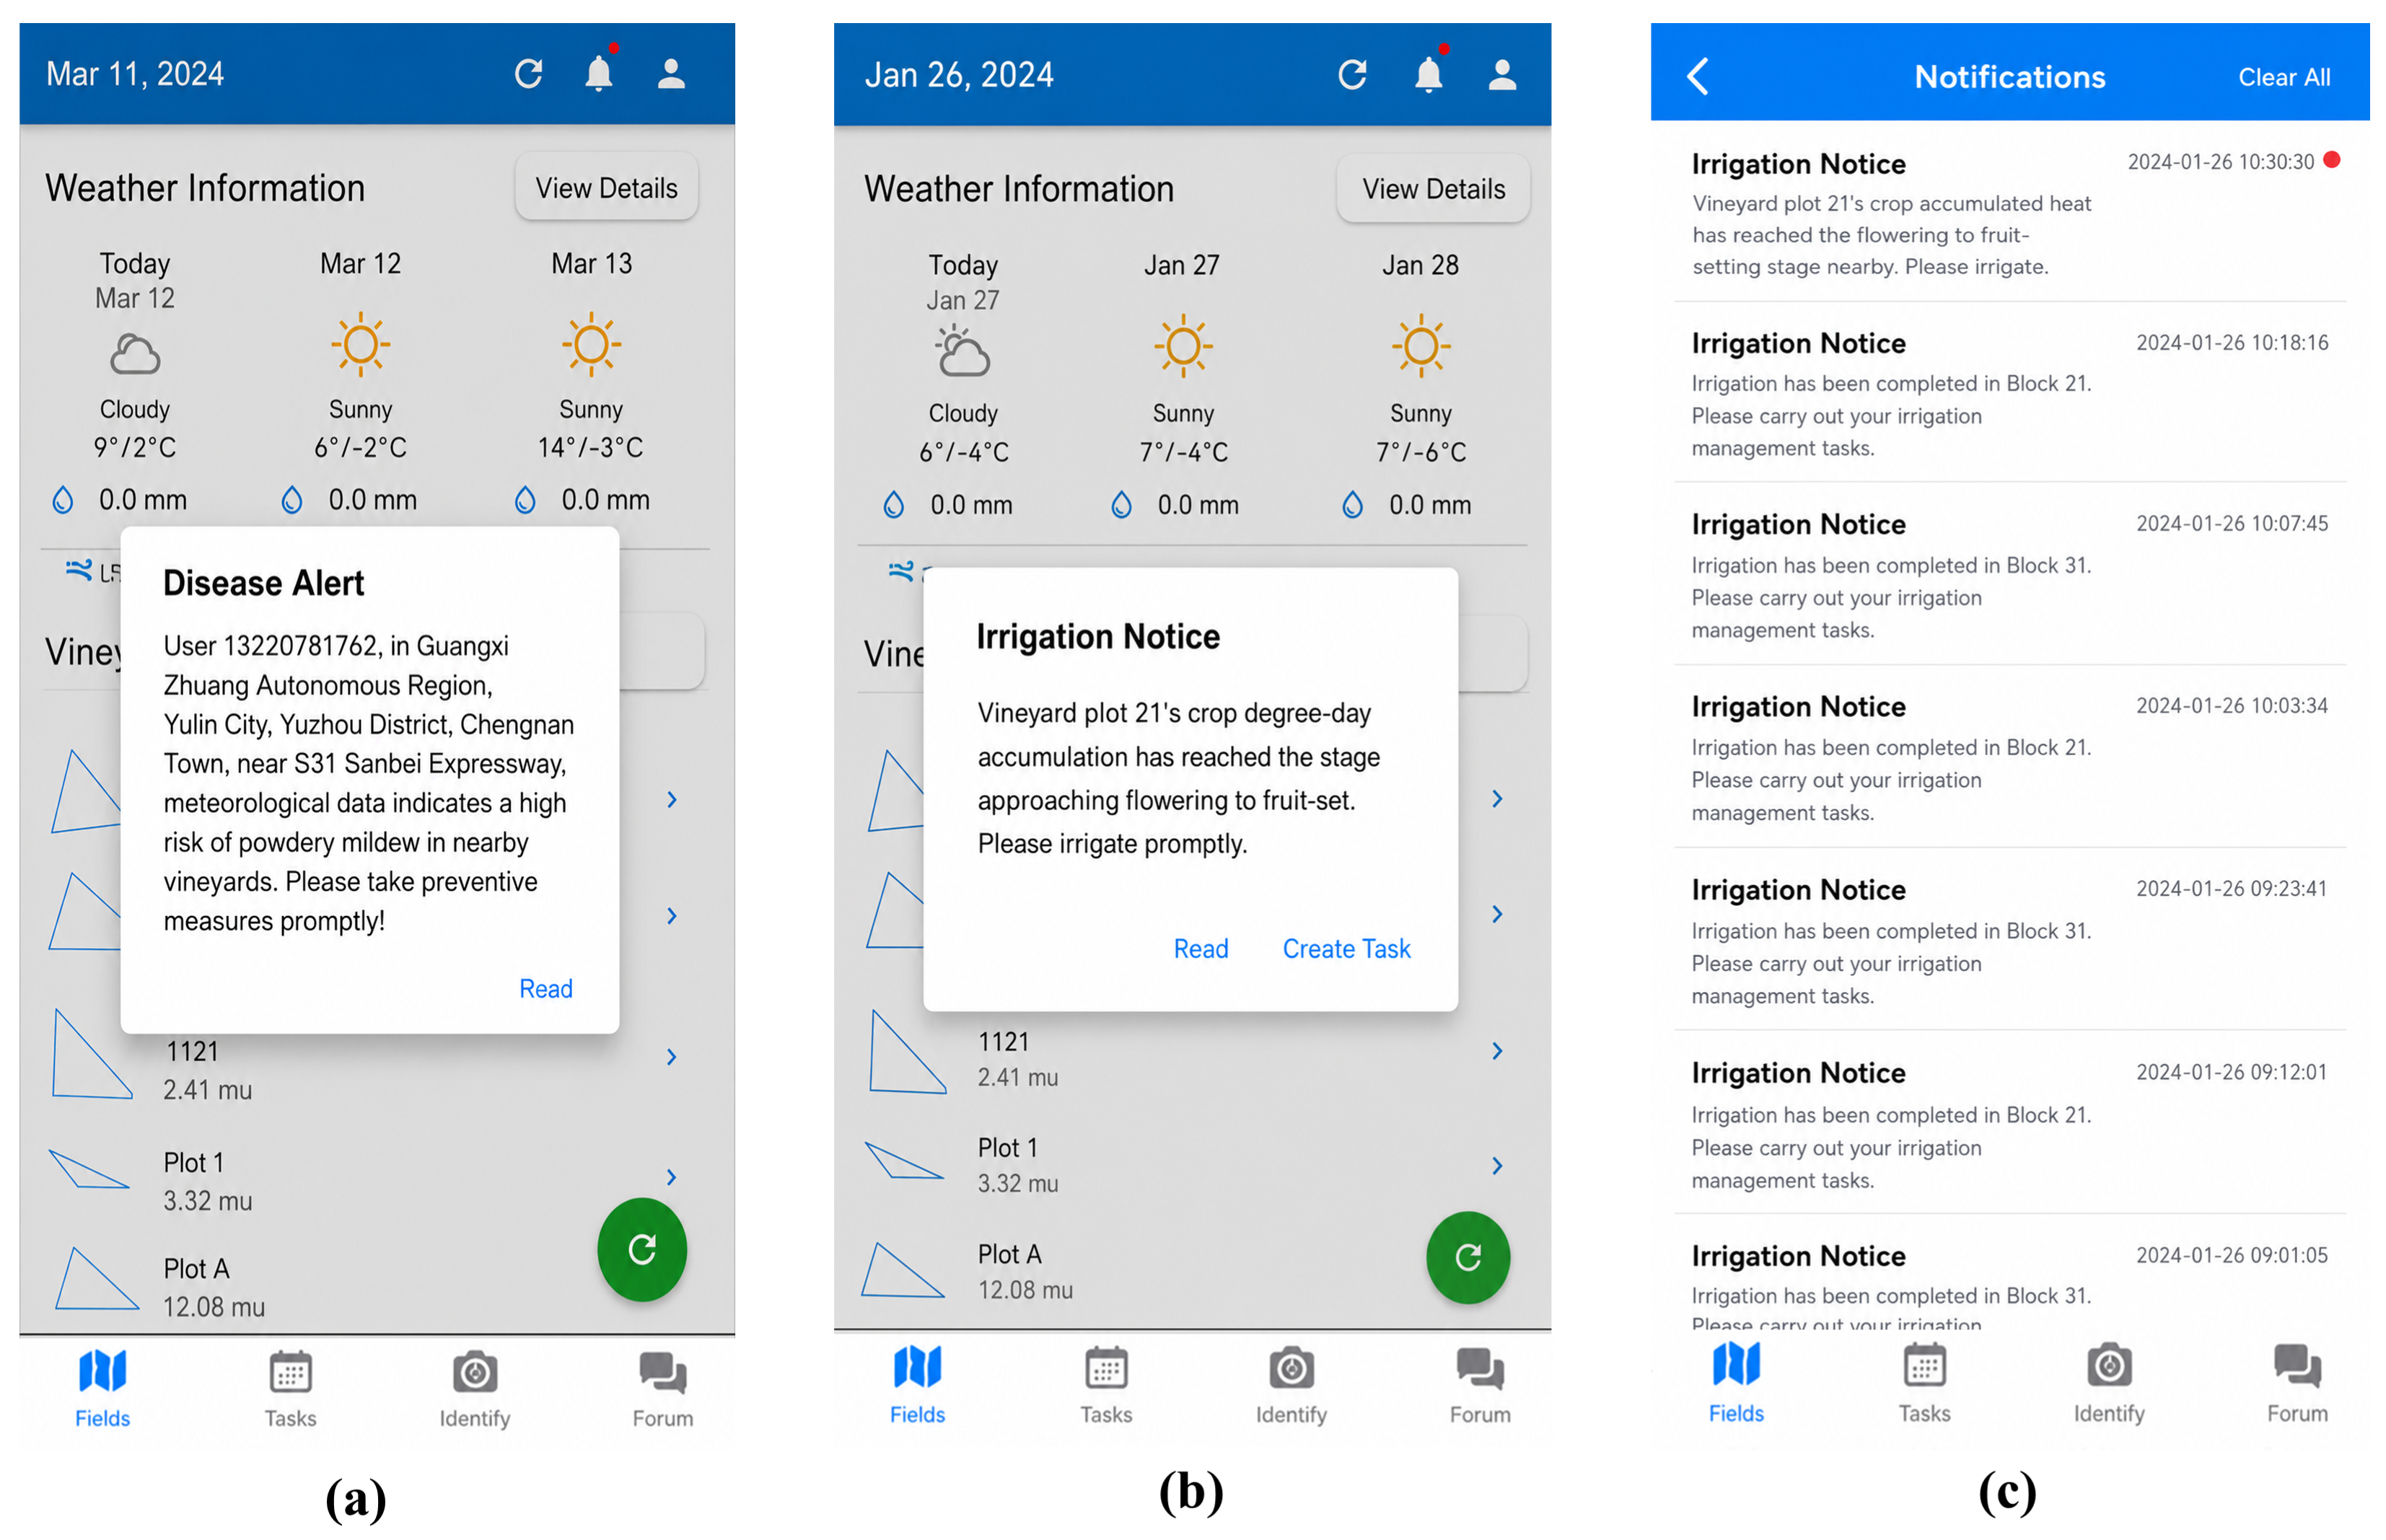
\includegraphics[width=\linewidth]{../fig/alert_notification_interfaces.png}
\caption[Warning and notification functions]{Warning and notification functions in GrapeMaster. (a) Disease-risk alert. (b) Management reminder. (c) Notification archive.}
\label{fig:alert_notification_interfaces_result}
\end{figure}

\begin{figure}[H]
\centering
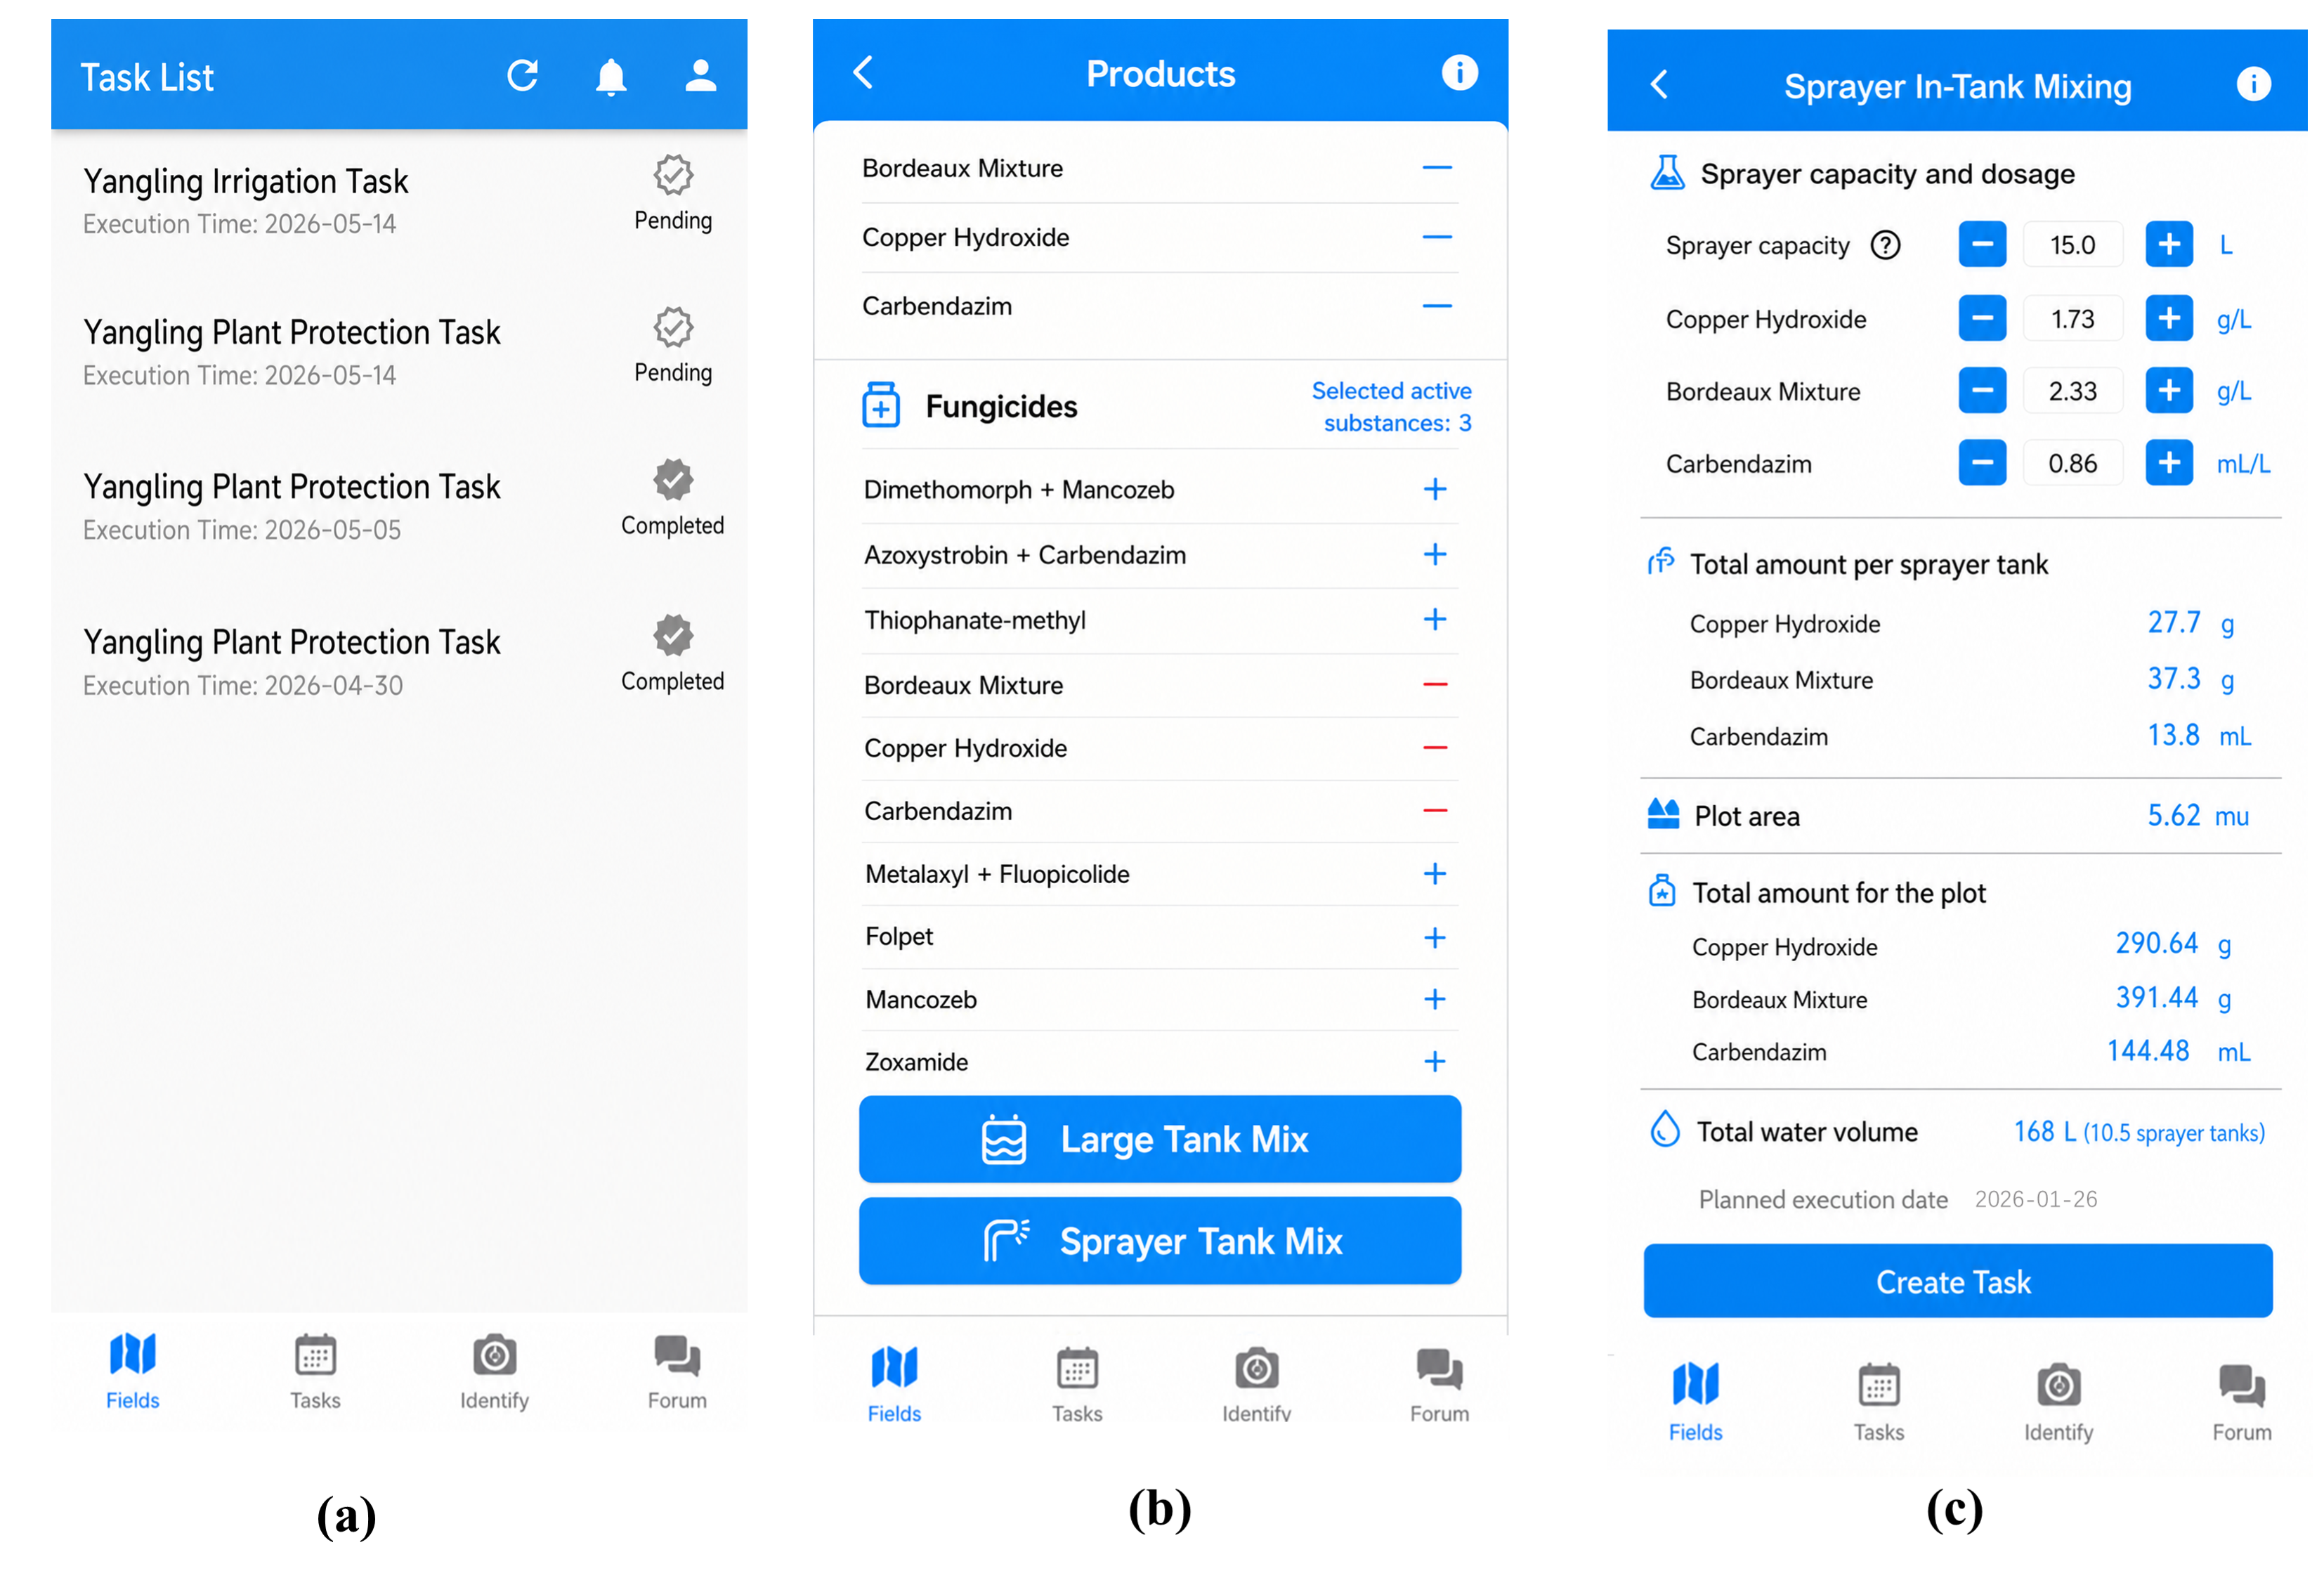
\includegraphics[width=\linewidth]{../fig/task_management_interfaces.png}
\caption[Task and treatment-recording functions]{Task and treatment-recording functions in GrapeMaster. (a) Field-operation list and status. (b) Product selection linked to a plant-protection task. (c) Tank-mixing calculation using sprayer capacity, dosage, plot area, water volume, and planned date.}
\label{fig:task_management_interfaces_result}
\end{figure}

\subsection{Post-symptomatic diagnostic and advisory workflow}\label{symptom-image-and-advisory-functions}

The post-symptomatic workflow allowed users to upload a field image, receive a disease class and confidence value, and continue to a conversational advisory interface (Figure~\ref{fig:ai_diagnosis_interfaces_result}). The mobile application displayed recognition output and retained user questions and returned advisory messages. This workflow complemented the proactive disease model: image recognition addressed visible symptoms, while the LLM supported interpretation and follow-up interaction. Advisory messages were not treated as autonomous treatment prescriptions, and their agronomic quality was not independently evaluated in this study.

\begin{figure}[H]
\centering
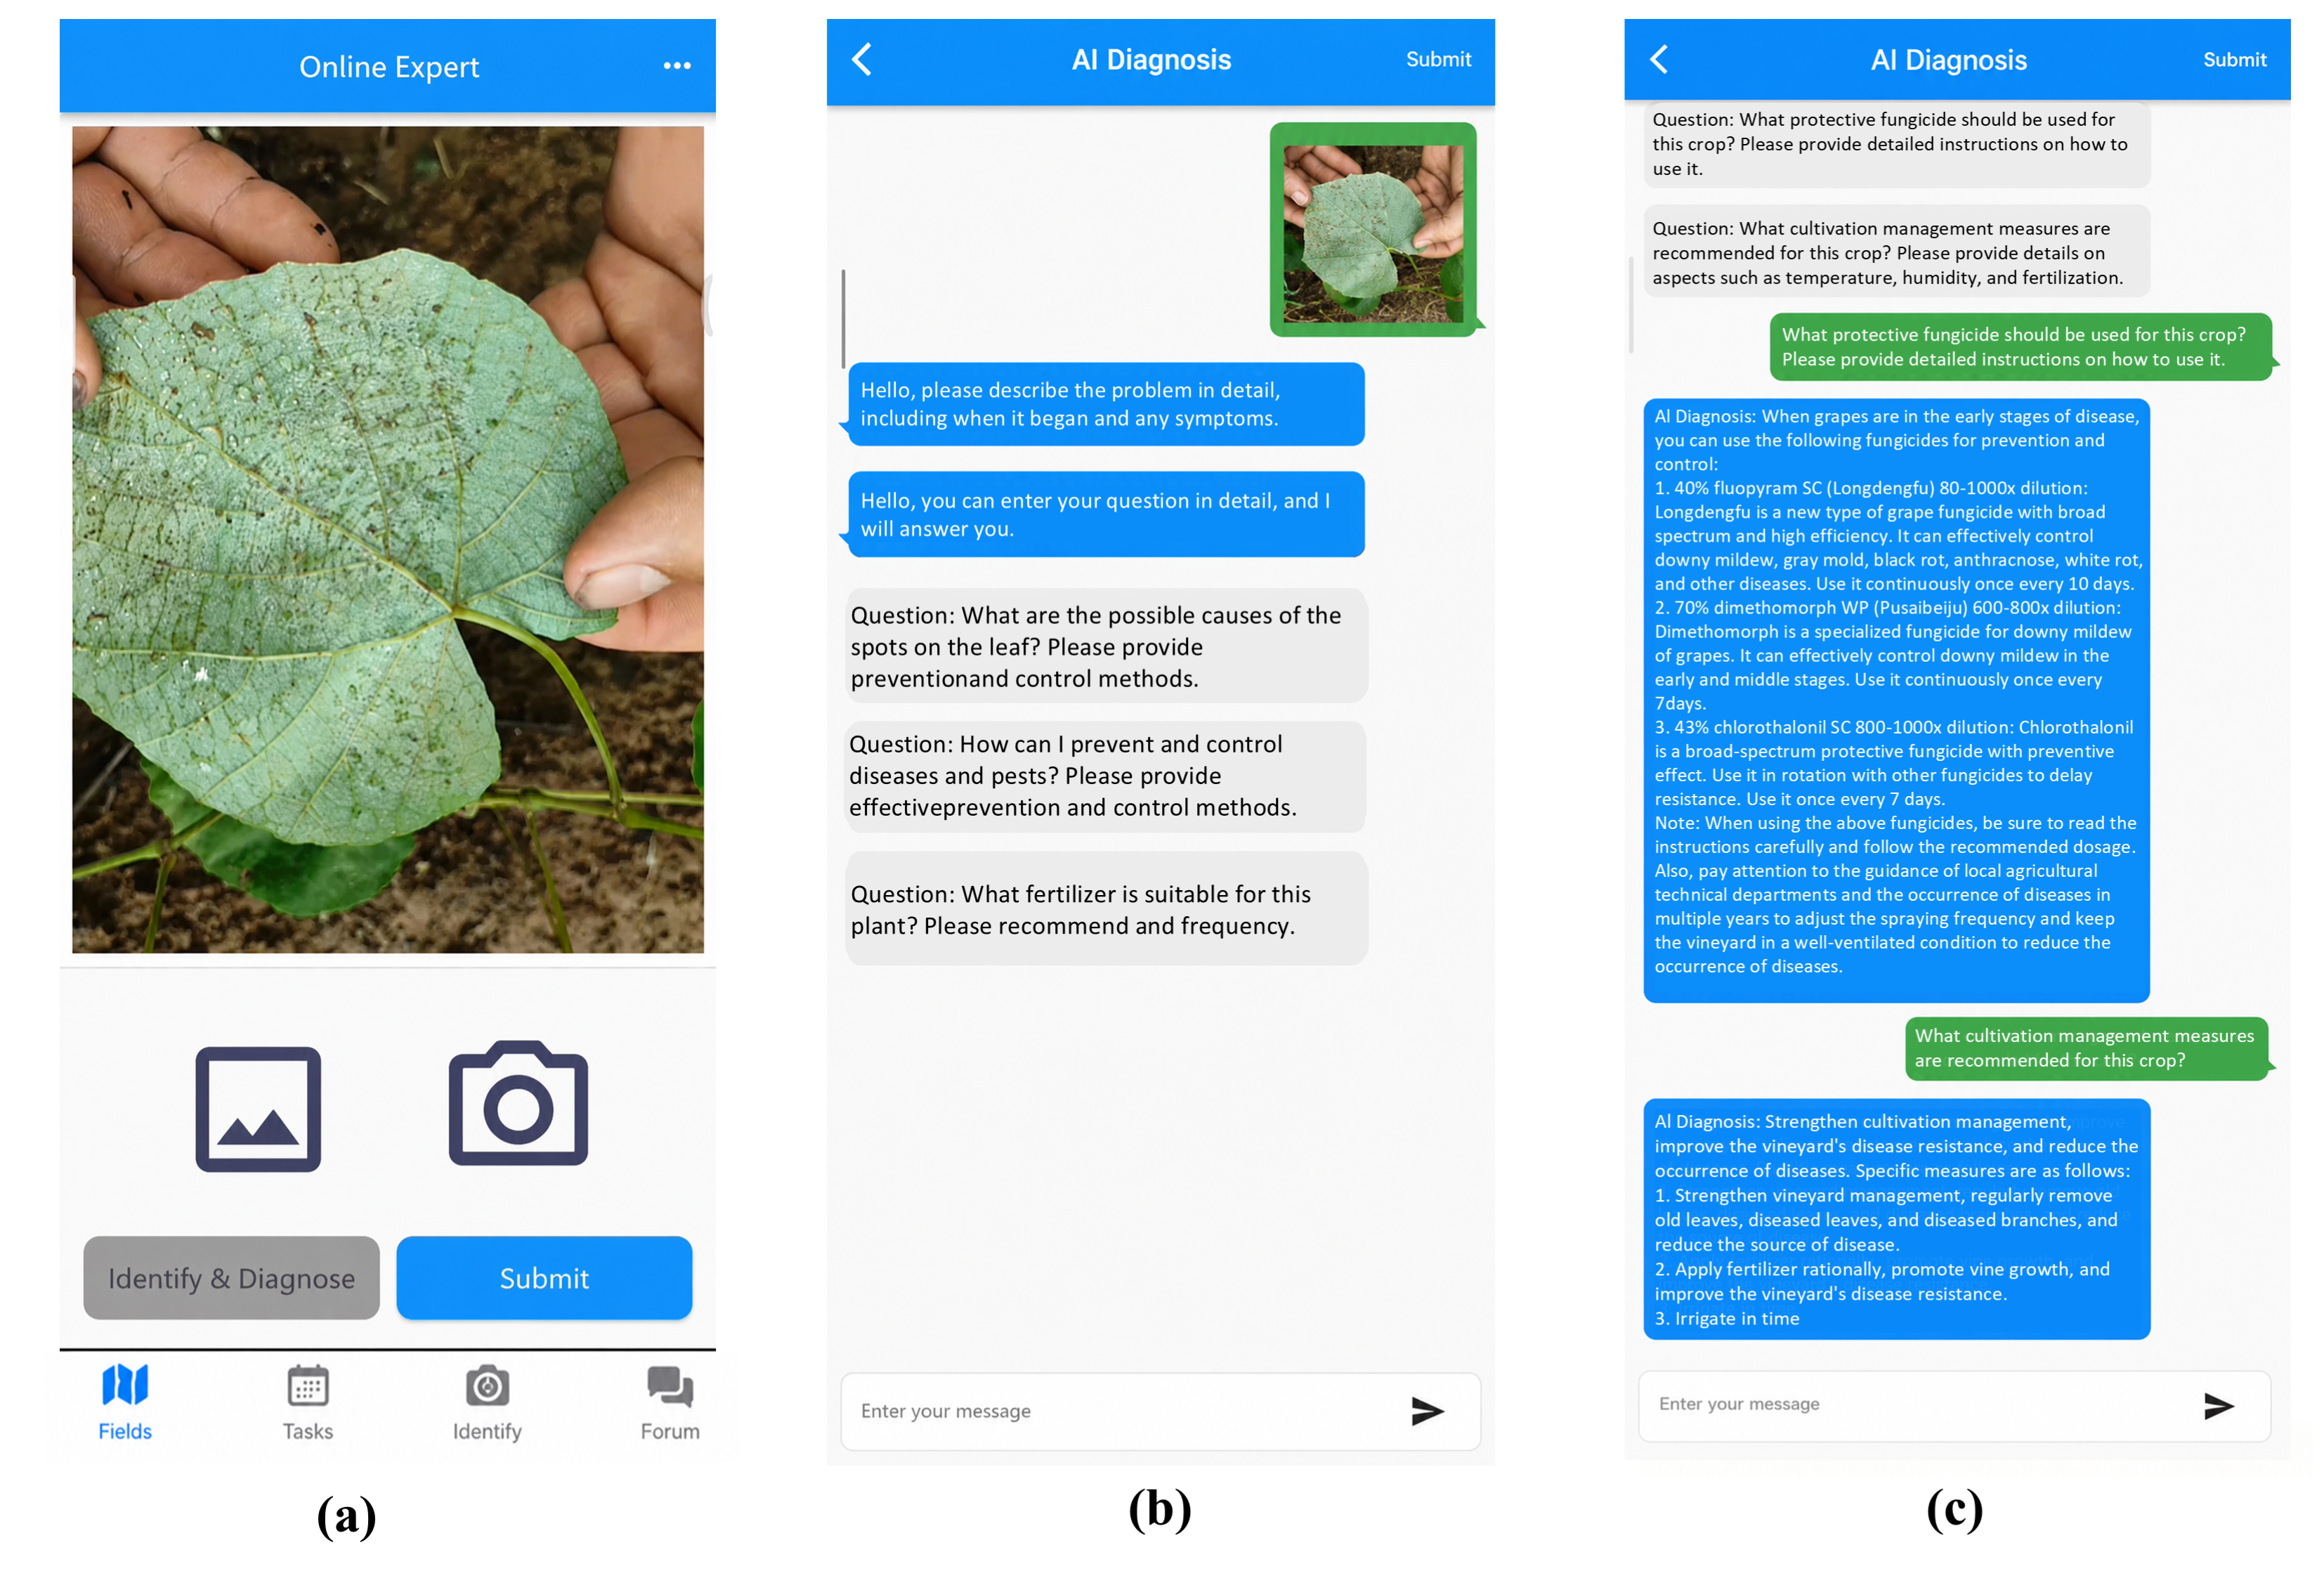
\includegraphics[width=\linewidth]{../fig/ai_diagnosis_interfaces.png}
\caption[Image-recognition and advisory interfaces]{Image-recognition and advisory interfaces in GrapeMaster. (a) Symptom-image upload. (b) Advisory entry associated with the uploaded image. (c) Conversational management-oriented response.}
\label{fig:ai_diagnosis_interfaces_result}
\end{figure}

\subsection{Deployment demonstration}\label{deployment-and-backend-record-audit}

The exported records spanned 2023--2026. After deduplication, 47 of 95 registered accounts contained both field-creation and crop-management records and were retained as operational accounts. These accounts contained 139 vineyard fields and 128 crop-management records. The export further contained 126 weather records, 126 phenology records, 252 disease-risk and model request--response records, 3,590 notifications, 151 plant-protection or irrigation tasks, and 234 fungicide or pesticide records. Symptom and advisory functions generated 94 field-note or disease-report records, 2,808 image-analysis records, 1,360 advisory or message records, and 27 forum records (Table~\ref{tab:backend_operational_coverage}).

The representative case contained weather, phenology, disease-risk, notification, completed plant-protection task, and fungicide-product records (Figure~\ref{fig:crop_season_replay_loop}; Supplementary Table S4). Environmental and analytical records shared a crop-management identifier, and product records were linked directly to tasks. The replay reconstructed the implemented sequence from state updating and risk interpretation to event delivery, operation recording, and treatment feedback. No field observation or disease-incidence record was available for this case. Accordingly, the replay demonstrates record-level implementation and contextual continuity, not that the warning caused the task or that the treatment improved disease outcomes.

\begin{table}[H]
\centering
\begingroup
\setlength{\tabcolsep}{3pt}
\renewcommand{\arraystretch}{1.12}
\scriptsize
\caption{Operational records retained from the deployed GrapeMaster backend.}
\label{tab:backend_operational_coverage}
\begin{minipage}{0.98\linewidth}
\begin{tabular}{p{0.21\linewidth} p{0.30\linewidth} p{0.22\linewidth} p{0.18\linewidth}}
\toprule
Record group & Retained records & Linkage basis & Demonstrated function \\
\midrule
Operational accounts & 47 of 95 deduplicated accounts & Account with at least one field and crop record & Implemented user workflow available for inspection \\
Field and crop context & 139 fields and 128 crop-management records & Account, field UUID, and crop UUID & Spatial and time-dependent management context \\
Environmental and analytical state & 126 weather, 126 phenology, and 252 risk/request--response records & Shared crop UUID & Model inputs and outputs retained for retrieval \\
Events and operations & 3,590 notifications and 151 plant-protection or irrigation tasks & User, field, or crop context & Delivery and field-operation functions retained \\
Treatment feedback & 234 product records linked to 141 plant-protection tasks & Task UUID & Product applications connected directly to tasks \\
Symptom and advisory records & 94 notes/reports, 2,808 image analyses, 1,360 messages, and 27 forum records & Account, field, crop, image, or message identifiers & Diagnostic and advisory functions retained with varying contextual completeness \\
Interpretation boundary & No controlled production comparison & Not applicable & No efficacy, adoption, pesticide-reduction, or economic outcome inferred \\
\bottomrule
\end{tabular}
\par\vspace{0.25em}{\raggedright\scriptsize Abbreviation: UUID, universally unique identifier.\par}
\end{minipage}
\endgroup
\end{table}

\begin{figure}[H]
\centering
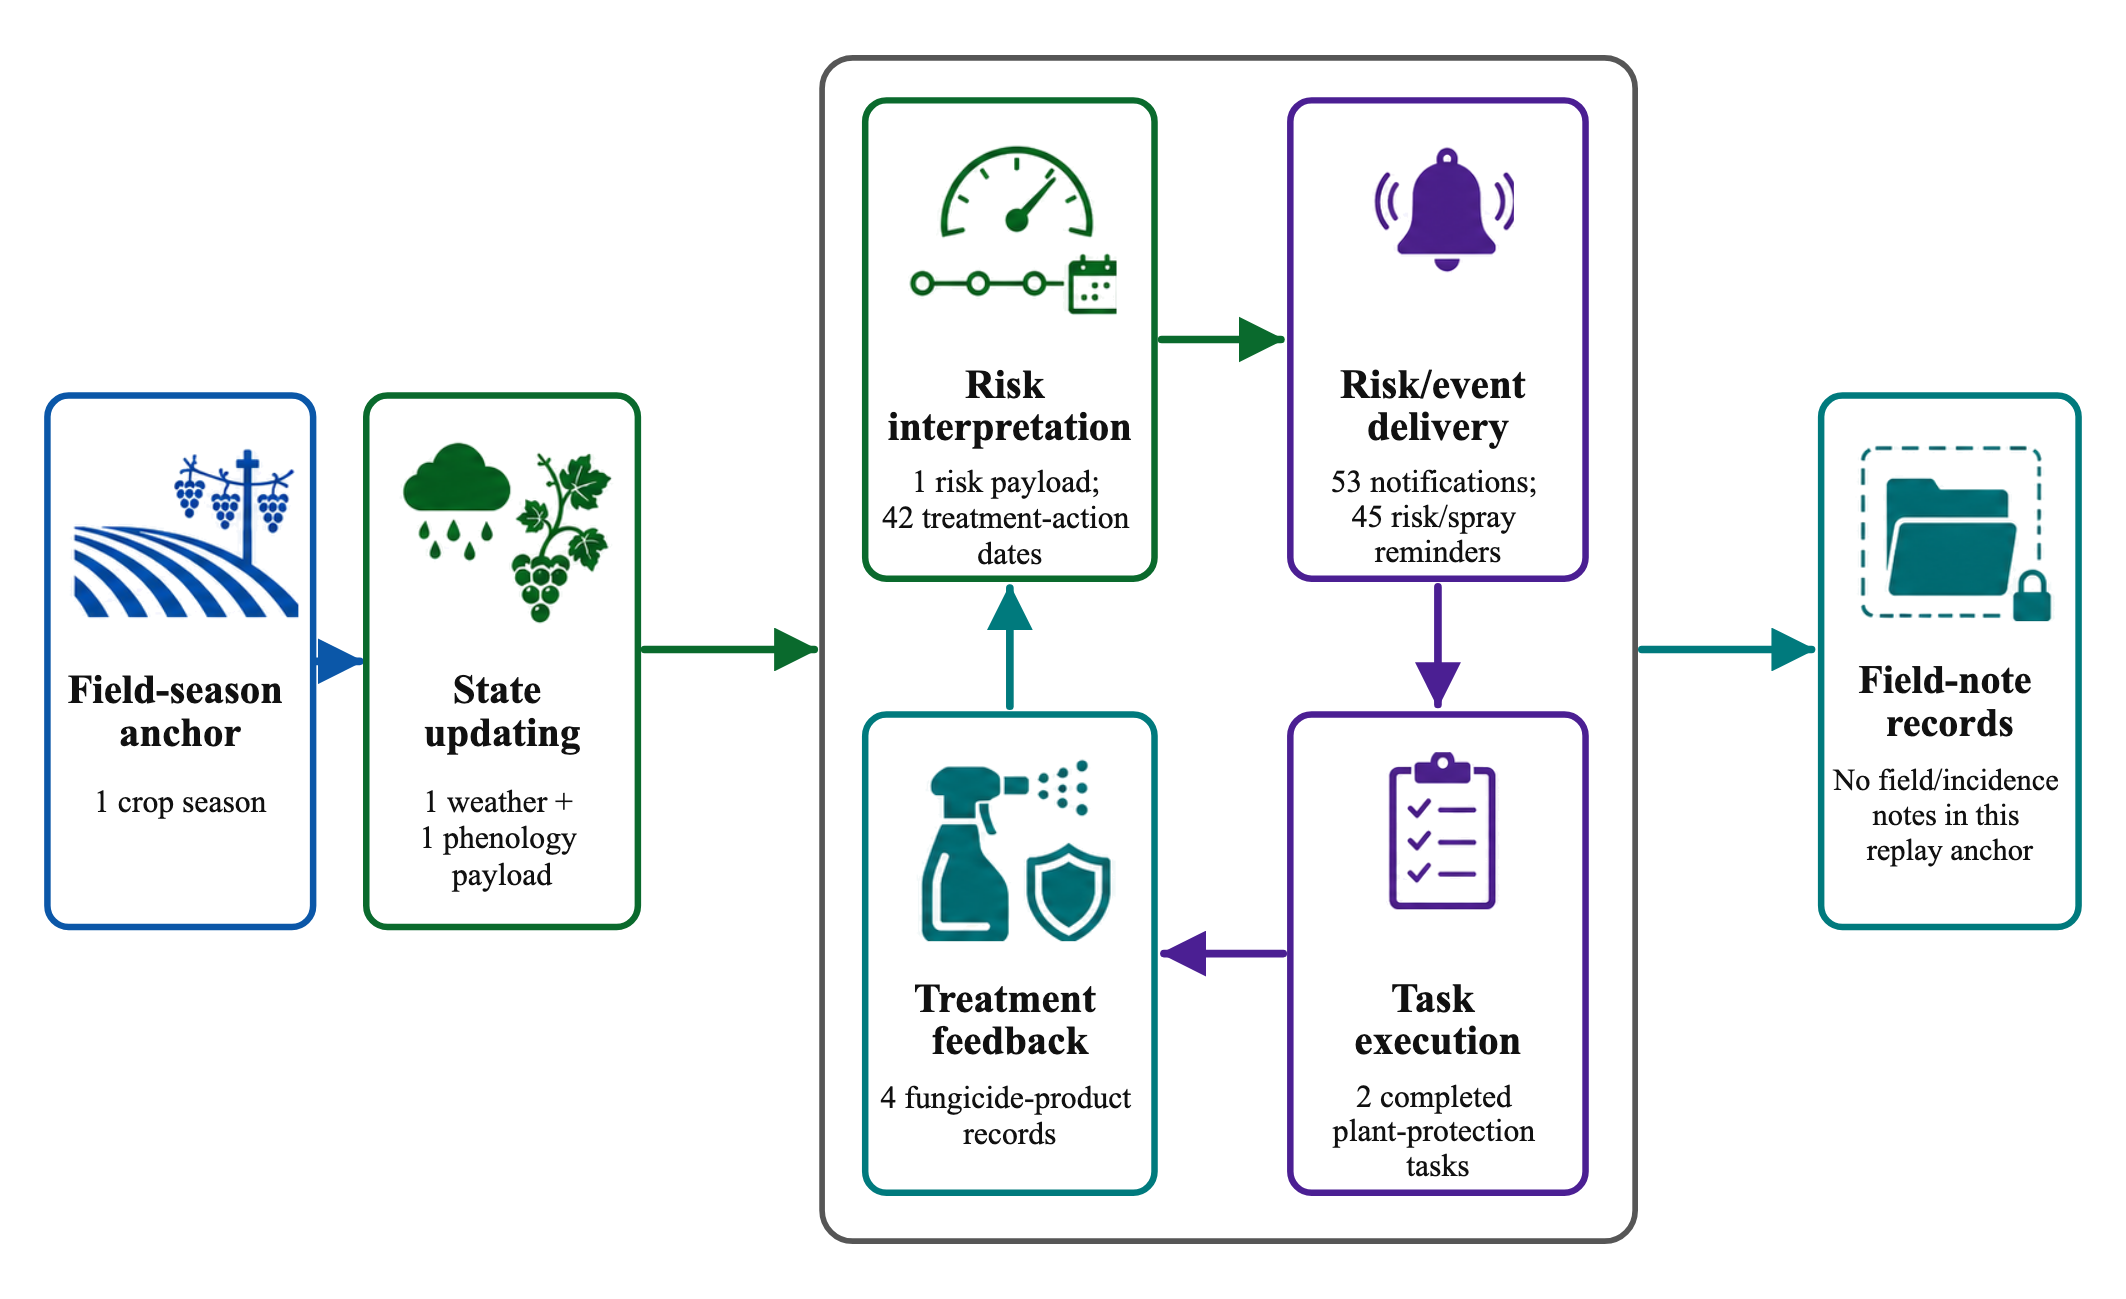
\includegraphics[width=\linewidth]{../fig/disease_feedback_loop_frame_balanced_revised_figure_package/disease_feedback_loop_frame_balanced_revised_300dpi.png}
\caption[Record-level replay of the risk-to-feedback workflow]{Record-level replay of the risk-to-feedback workflow in GrapeMaster. Node labels show retained records in the representative case. Shared crop context connects environmental, analytical, notification, and task records; task identifiers directly connect applied products to field operations.}
\label{fig:crop_season_replay_loop}
\end{figure}

\subsection{Supporting performance of analytical components}\label{evaluation-of-platform-compatible-analytical-modules}

The component evaluations used Guangxi field observations and a labeled grape disease image dataset (Table~\ref{tab:guangxi_field_data}). These results characterize bounded analytical readiness and are not interpreted as evidence of complete software effectiveness or production outcomes.

For the Guangxi broad-stage phenology module, the evaluation used 151 valid field observations from six Guangxi site-years. The module reached 58.0\% exact major-stage agreement and 76.0\% user-visible agreement after transition-window display, with a mean absolute stage distance of 0.45 major stages when the sparse post-harvest class was excluded from core metrics (Figure~\ref{fig:phenology_major_stage_validation_result}).

For the downy mildew risk-warning module, the FSIM-S configuration produced a validation mean absolute error of 6.3 days and a validation root mean square error of 6.5 days for first-infection timing (Figure~\ref{fig:core_analytical_support_result}). This result describes the evaluated Guangxi configuration of the platform-compatible risk module rather than the effectiveness of deployed plant-protection decisions.

For the grape disease image-recognition module, the evaluated model produced class-wise F1-scores from 0.926 to 0.998 across seven grape disease categories, with downy mildew reaching an F1-score of 0.986 (Figure~\ref{fig:core_analytical_support_result}). The LLM-assisted advisory component was integrated into the application but was not included in component evaluation because no independent result for advisory quality was available.

\begin{table}[H]
\centering
\caption{Datasets used for supporting analytical-component evaluation.}
\label{tab:guangxi_field_data}
\tablefontsize
\begin{tabular}{@{}p{0.24\linewidth} p{0.23\linewidth} p{0.16\linewidth} p{0.29\linewidth}@{}}
\toprule
Site or dataset & Cultivar or scope & Years & Data types \\
\midrule
Mingyang, Nanning & Jufeng & 2023, 2024 & Phenology observations, downy mildew monitoring, airborne sporangia monitoring, and management records \\
Du'an, Hechi & Maoputao Yeniang No. 2 & 2022, 2023, 2024 & Phenology observations, downy mildew monitoring, airborne sporangia monitoring, and management records \\
Xing'an, Guilin & Wenke & 2022 & Phenology observations, downy mildew monitoring, airborne sporangia monitoring, and management records \\
Grape disease image dataset & Seven grape disease categories & Not site-year based & Labeled symptom images \\
\bottomrule
\end{tabular}
\end{table}

\begin{figure}[H]
\centering
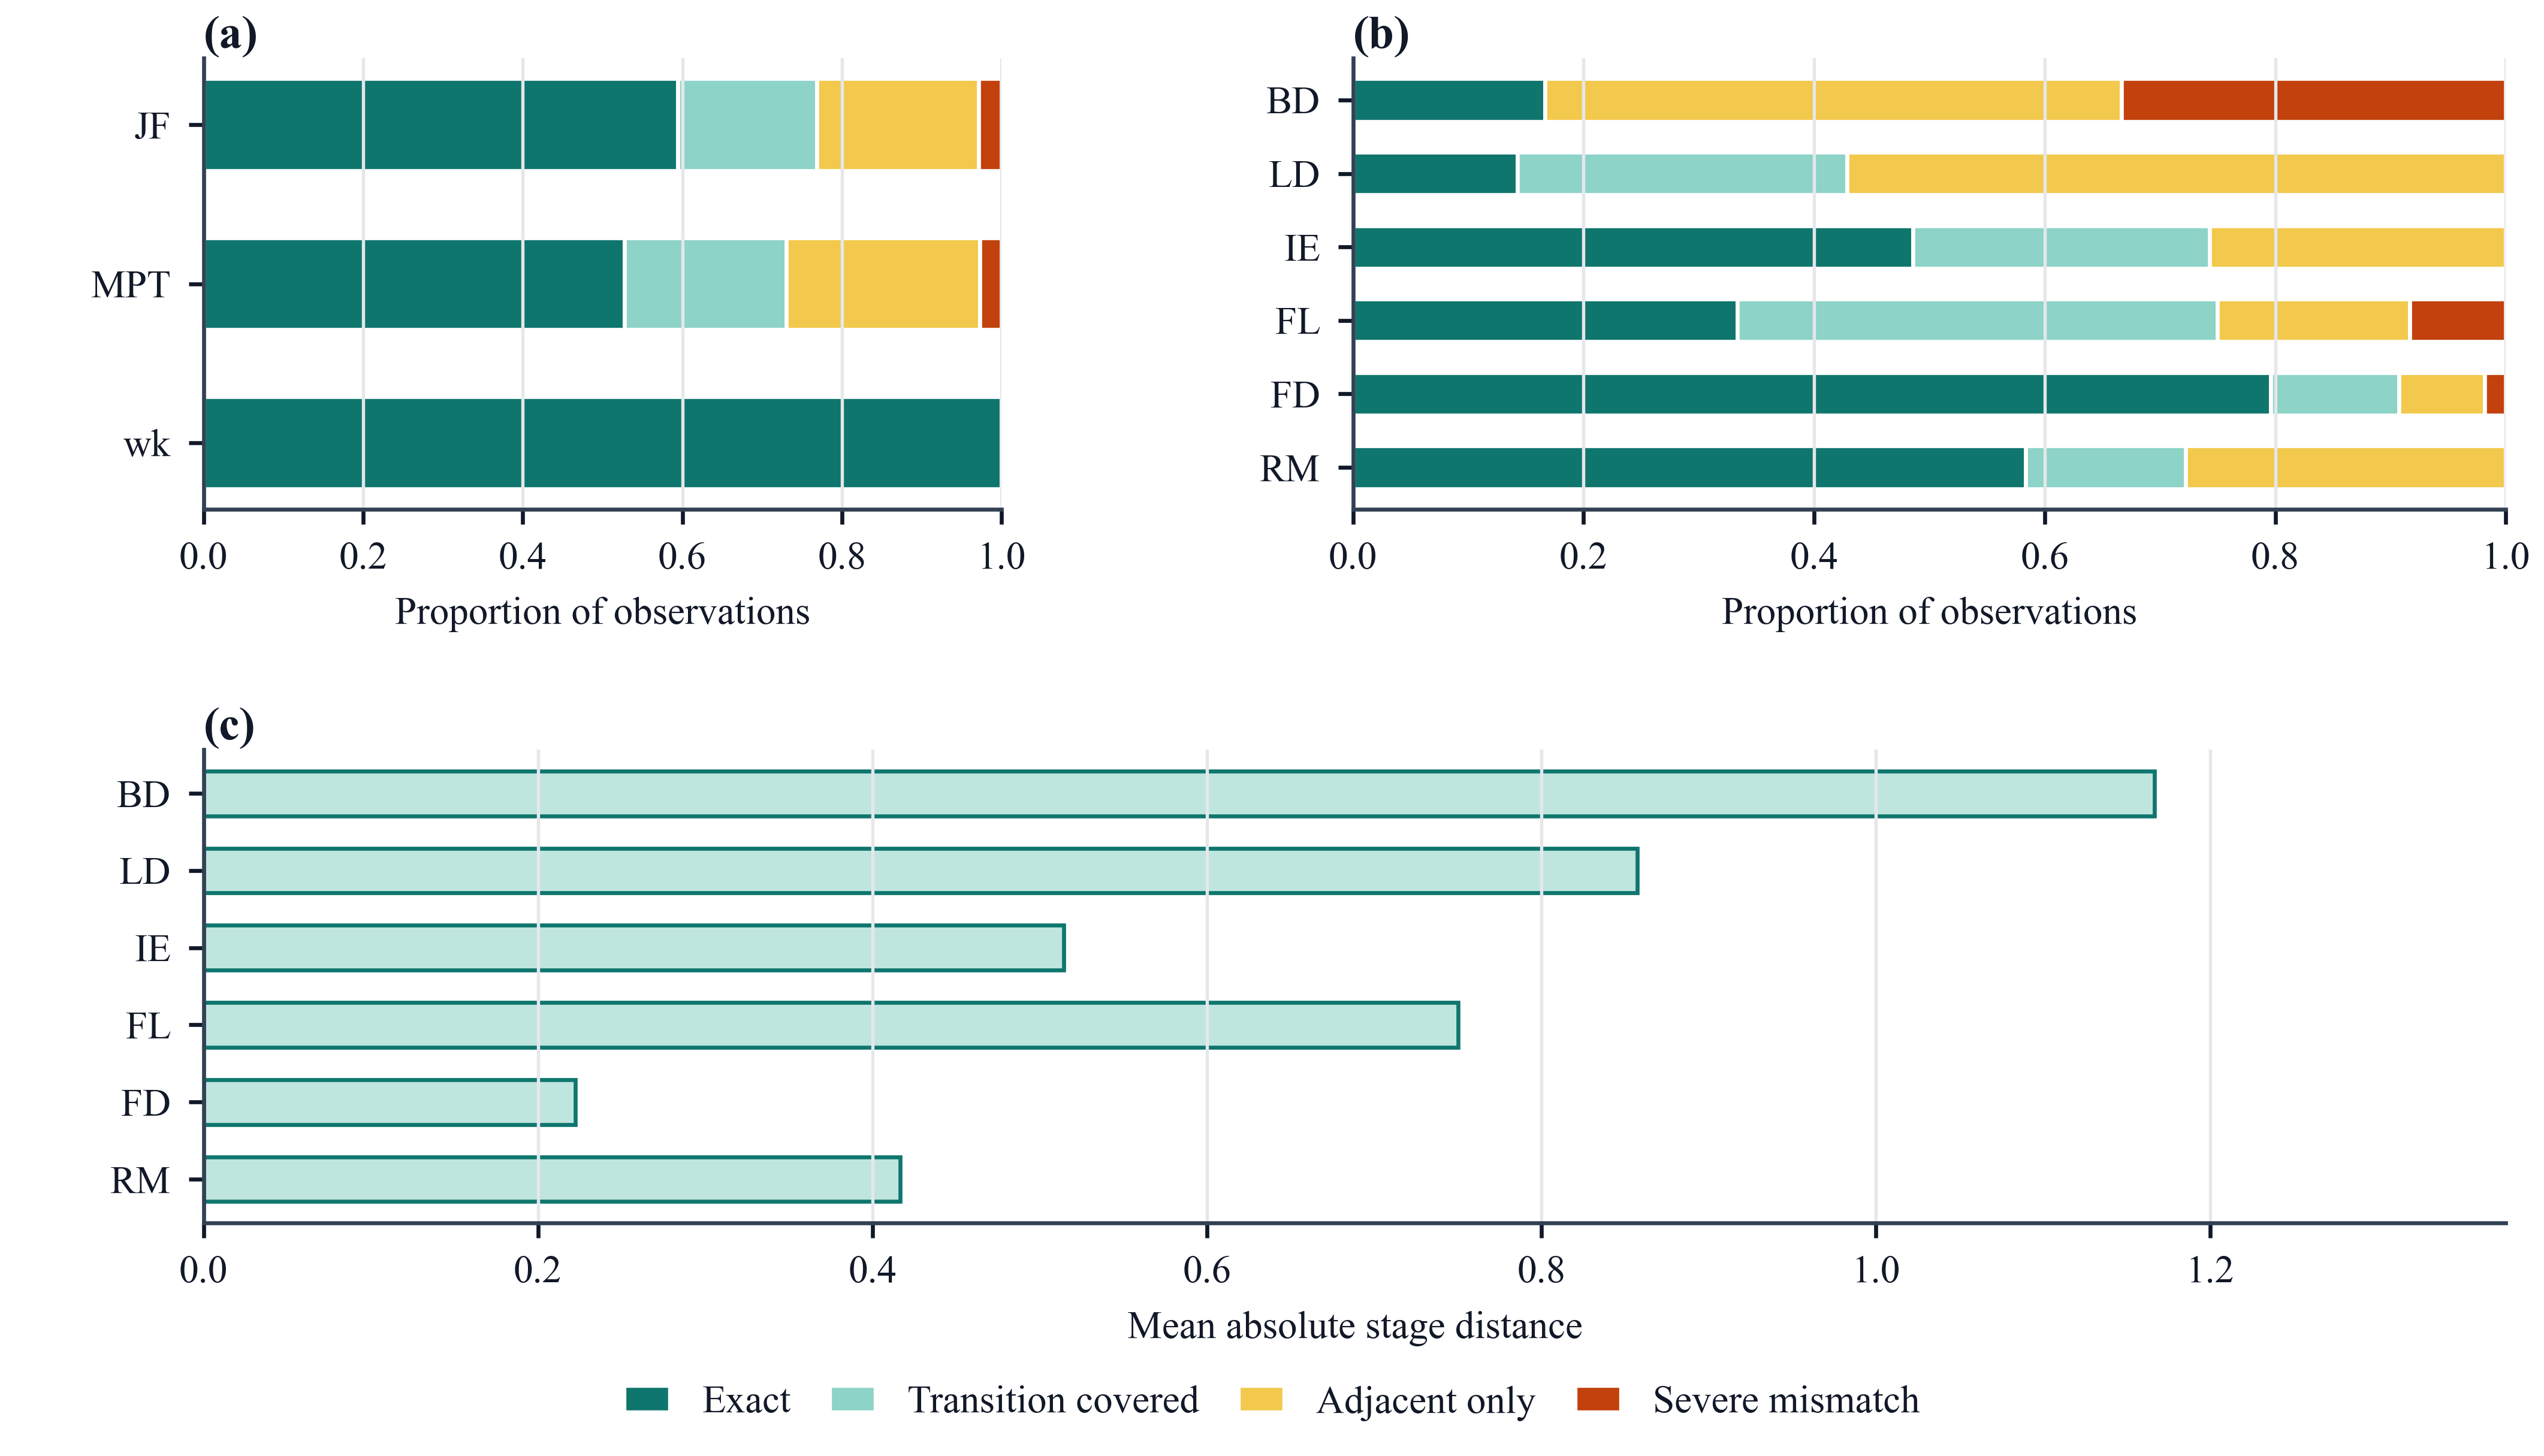
\includegraphics[width=\linewidth]{../fig/phenology_major_stage_validation.png}
\caption[Validation of the broad-stage phenology component]{Validation of the broad-stage phenology component. (a) Outcome proportions by cultivar. (b) Outcome proportions by observed major stage. (c) Mean absolute stage distance by observed major stage. BD, bud development; LD, leaf development; IE, inflorescence emergence; FL, flowering; FD, fruit development; RM, ripening of berries.}
\label{fig:phenology_major_stage_validation_result}
\end{figure}

\begin{figure}[H]
\centering
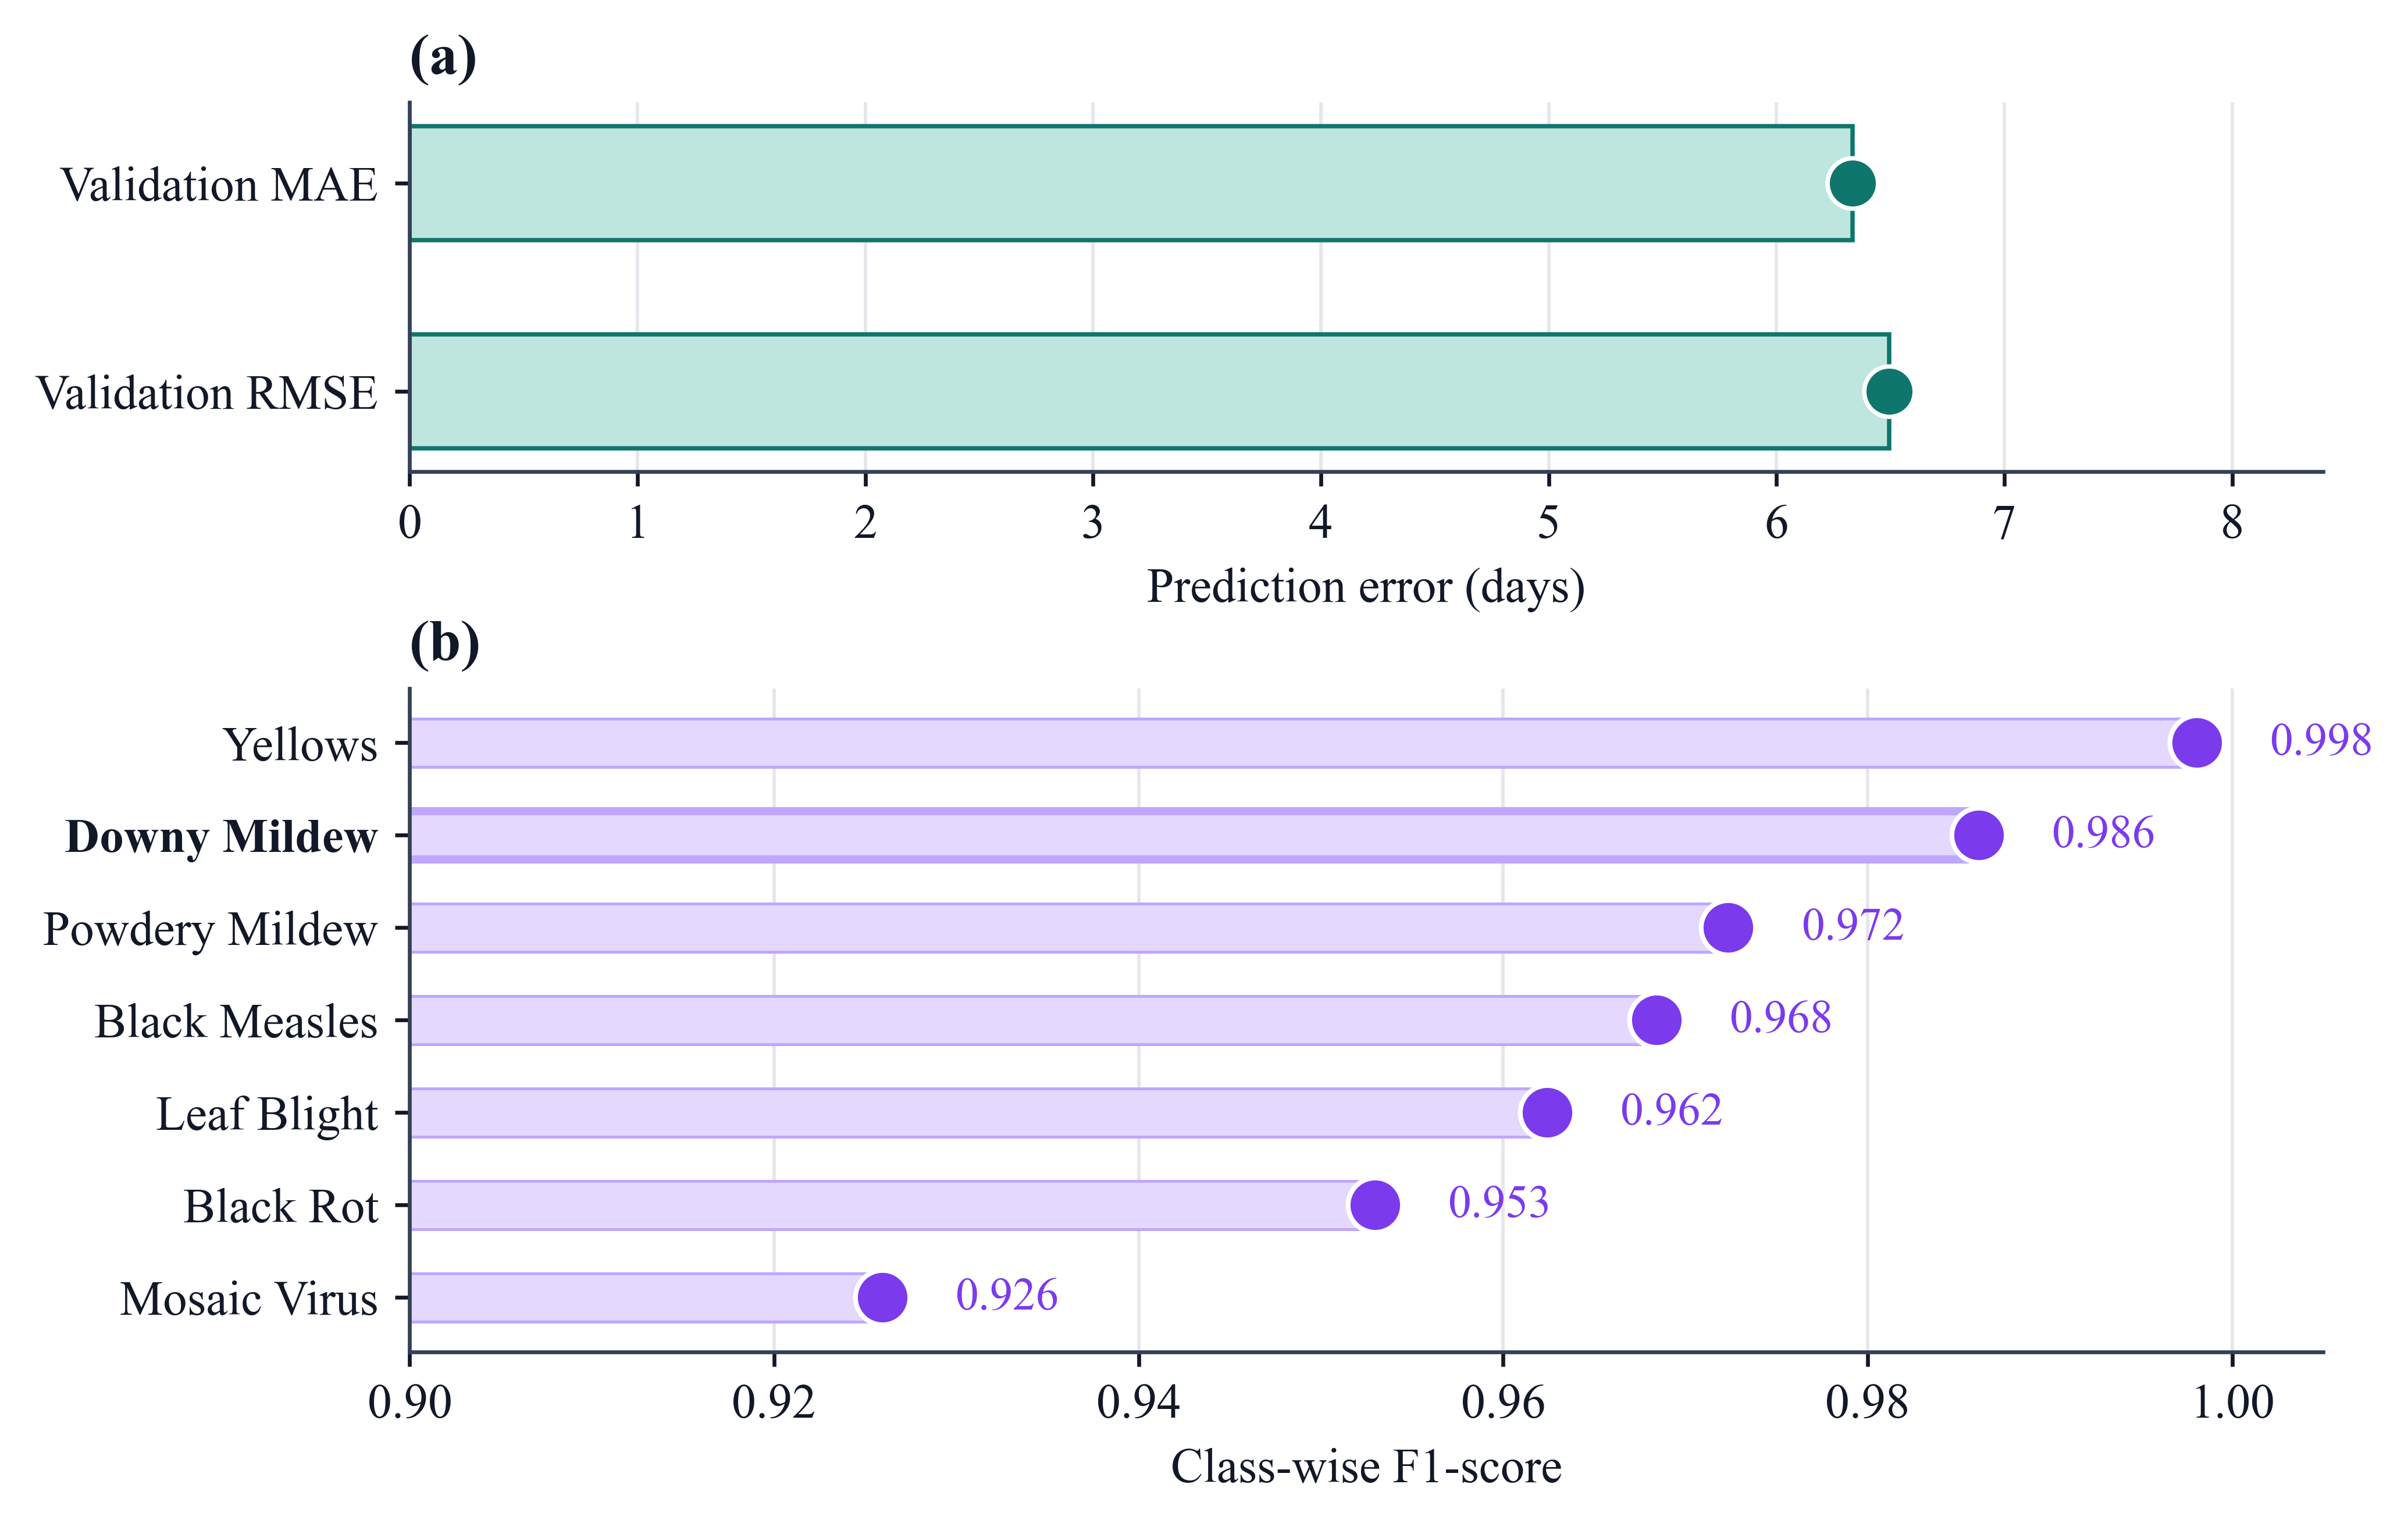
\includegraphics[width=\linewidth]{../fig/fsims_supporting_performance.png}
\caption[Supporting disease-model and image-recognition results]{Supporting analytical-component results. (a) Validation error for FSIM-S downy mildew first-infection timing. (b) Class-wise image-recognition F1-scores, with downy mildew highlighted.}
\label{fig:core_analytical_support_result}
\end{figure}

\section{Discussion}\label{discussion}

\subsection{From isolated outputs to operational disease-management intelligence}\label{operational-disease-management-intelligence}

The principal contribution of GrapeMaster is not the co-location of several functions in one mobile application. It is the software path by which heterogeneous analytical outputs become persistent and actionable management information. Environmental and phenological processing supplies the changing context for pre-symptomatic disease analysis; the backend persists requests and responses; the application presents risk and warning information; and management services retain tasks and products. The post-symptomatic branch adds image-based evidence and conversational interpretation. Together, these functions address the fragmentation described in the Introduction by assigning each analytical service an operational role.

This integration is particularly relevant for disease management because an analytical result has limited value when it cannot be related to the intervention history that affects its later interpretation \citep{rossiAddressingImplementationProblem2014,rossiSharingDecisionmakingTools2023}. GrapeMaster therefore treats model execution, result delivery, and operation recording as connected software concerns. The crop-management identifier assists record retrieval, but it is the orchestration logic---not the identifier itself---that creates the integrated workflow.

\subsection{Orchestrating heterogeneous analytical services}\label{orchestrating-analytical-services}

The integrated services operate differently. Weather and phenology are refreshed by scheduled backend jobs; disease forecasting requires a structured, date-aligned request; image recognition is triggered by an uploaded image; and LLM advisory is interactive and message based. A common presentation layer alone cannot reconcile these patterns. GrapeMaster uses backend-owned business objects and service interfaces to coordinate them while preserving model-specific inputs and outputs.

The resulting modularity is bounded by interface quality. A disease model can be recalibrated or replaced if its request and response contract remains compatible, and a hosted image or language model can be updated without rewriting field and task management. However, reproducibility requires the deployed service version, configuration, checkpoint, and data contract to be archived. The module results reported here show that independently developed analytical components can support the platform, but they do not establish that every compatible service is valid in every region. Local calibration and validation remain necessary \citep{bregaglioPublicDecisionSupport2022}.

\subsection{Connecting risk interpretation with treatment feedback}\label{from-analytical-outputs-to-executable-disease-management-records}

Treatment feedback is the clearest example of model-to-management integration in GrapeMaster. A completed plant-protection task does not remain only as a note: the backend translates product and execution information into the treatment-history structure accepted by the disease service and can initiate renewed analysis. This design allows risk to be interpreted with knowledge of recent management, reflecting the temporary protection expected from fungicide application \citep{caffiFungicideModelsAre2018,warnekeEffectFungicideMobility2020}.

The implementation should nevertheless be interpreted carefully. Product-to-task linkage is direct, whereas a notification and a subsequently created task may be connected only by shared user, field, or crop context. The deployment replay therefore supports reconstruction of a risk-to-action-to-feedback sequence but not a causal claim that a specific warning produced a specific treatment. Adding explicit provenance fields for source event, user decision, and resulting analytical update would strengthen future versions.

\subsection{Relationship to agricultural decision-support platforms}\label{relationship-to-existing-platforms}

Existing vineyard DSSs demonstrate the importance of monitoring, disease-model delivery, communication, and regional warning services \citep{rossiAddressingImplementationProblem2014,bregaglioPublicDecisionSupport2022}. GrapeMaster extends this line of work through the particular combination of proactive disease modeling, field-operation records, treatment-aware recalculation, post-symptomatic image recognition, and LLM-assisted interaction in a mobile/backend implementation. The claim is not universal superiority or the first use of each technology. The distinction lies in the explicit software path across predictive, diagnostic, advisory, and operational functions.

This system-level perspective is consistent with agricultural computing research that treats integration, service boundaries, data flow, and user interaction as part of the technical contribution \citep{fountasFarmManagementInformation2015,romera2024digitalization,bakirScalableEndtoendIoT2026}. It also changes the role of component validation: phenology, disease-risk, and image-recognition metrics establish bounded analytical readiness, whereas operational records demonstrate that the intended software objects and workflows were instantiated.

\subsection{Limitations and future work}\label{limitations-and-future-directions}

Several limitations remain. First, the adjacent source repositories do not by themselves preserve every deployed dependency and configuration. A reproducible release will require the weather provider, disease-service configuration, image-classification checkpoint, LLM checkpoint, prompts or context rules, and API versions to be archived together. Second, the current data model provides contextual rather than direct causal linkage for some transitions, especially notification to task and advisory interaction to subsequent field action. Third, the LLM advisory component was integrated but not independently evaluated for factual correctness, agronomic appropriateness, safety, or robustness.

Fourth, the deployment export demonstrates software use and record generation but does not measure usability, sustained adoption, disease-control efficacy, pesticide reduction, or economic benefit. Fifth, regional transfer requires recalibration and validation of analytical services for local cultivars, weather, and epidemiology. Future work should therefore add explicit event-to-action provenance, automated integration and failure-recovery tests, versioned model-service packages, independent LLM evaluation, usability studies, and controlled multi-region assessment of agronomic and economic outcomes.

\section{Conclusion}\label{conclusion}

GrapeMaster addresses the fragmentation of vineyard disease-management information by integrating analytical services with field operations in one mobile and backend software system. Its architecture connects scheduled environmental and phenological processing, pre-symptomatic disease-risk modeling, post-symptomatic image recognition, LLM-assisted advisory interaction, notifications, tasks, and treatment records through explicit application services and persistent data.

The central software contribution is the model-to-management orchestration mechanism. The backend constructs and retains analytical requests and responses, translates model output into user-facing management information, and transforms completed treatment records into inputs for subsequent disease-risk interpretation. Deployment records and a representative replay demonstrate that this workflow was implemented, while component evaluations provide bounded evidence for phenology, downy mildew, and image-recognition services.

GrapeMaster consequently offers a reusable approach for connecting predictive, diagnostic, advisory, and operational functions in agricultural decision-support software. Further development should strengthen service reproducibility, direct action provenance, LLM validation, usability evidence, and controlled evaluation of production outcomes.

\section*{CRediT authorship contribution statement}

To be completed before submission.

\section*{Declaration of competing interest}

The authors declare that they have no known competing financial interests or personal relationships that could have appeared to influence the work reported in this paper.

\section*{Data availability}

The de-identified derived datasets and analysis scripts supporting the figures, tables, and summary statistics reported in this study are available from the corresponding author upon reasonable request. These materials include operational-record summaries, representative workflow replay summaries, phenology validation results, disease-risk timeline data, figure source data, and the scripts used for data summarization and visualization.

Raw operational records from the deployed GrapeMaster platform are not publicly available because they contain user account information, field locations, uploaded images, messages, task records, and other management data subject to privacy and confidentiality restrictions. De-identified data supporting the reported analyses are available from the corresponding author upon reasonable request, subject to applicable privacy and confidentiality requirements.

\section*{Acknowledgements}

To be completed before submission.

\section*{Ethics and user data privacy statement}

The operational records used in this study were analyzed in aggregated or de-identified form, and no personally identifiable user information is reported.

\section*{Supplementary material}

Supplementary material associated with this article is provided as a separate file.

\bibliographystyle{elsarticle-harv}
\bibliography{../reference/Grape}

\end{document}
